\chapter{Results and Explainability}
\label{ch:results}

This chapter presents the evaluation of the CNN-Transformer model on the held-out test set, together with the full suite of explainability analyses and the detector robustness study. All results correspond to the six-stream architecture described in Chapter~\ref{ch:methodology}, which extends the three-stream CNN-Transformer model introduced in~\shortciteA{navarro2026transformer} with independent RAW attention streams per task, enabling attention maps at the level of individual detector hits. The test partition comprises 11,209 events and was withheld entirely during training and hyperparameter search. Section~\ref{sec:performance} reports quantitative performance across the three reconstruction tasks and compares them with the state of the art. Section~\ref{sec:explainability} presents two complementary feature importance analyses and the attention pattern study. Section~\ref{sec:robustness} quantifies model robustness to detector failures and derives first data-driven insights on array design.

% ============================================================
\section{Multi-Task Performance}
\label{sec:performance}
% ============================================================

Figure~\ref{fig:training_curves} shows the training and validation loss and metric curves across epochs. The model trained for 61 epochs before early stopping was triggered, with the best checkpoint at epoch 46 restored for evaluation. All three tasks converge jointly without any task dominating the optimization, and the gap between training and validation curves is narrow throughout, indicating that the regularization strategy is effective.

\begin{figure*}[ht!]
    \centering
    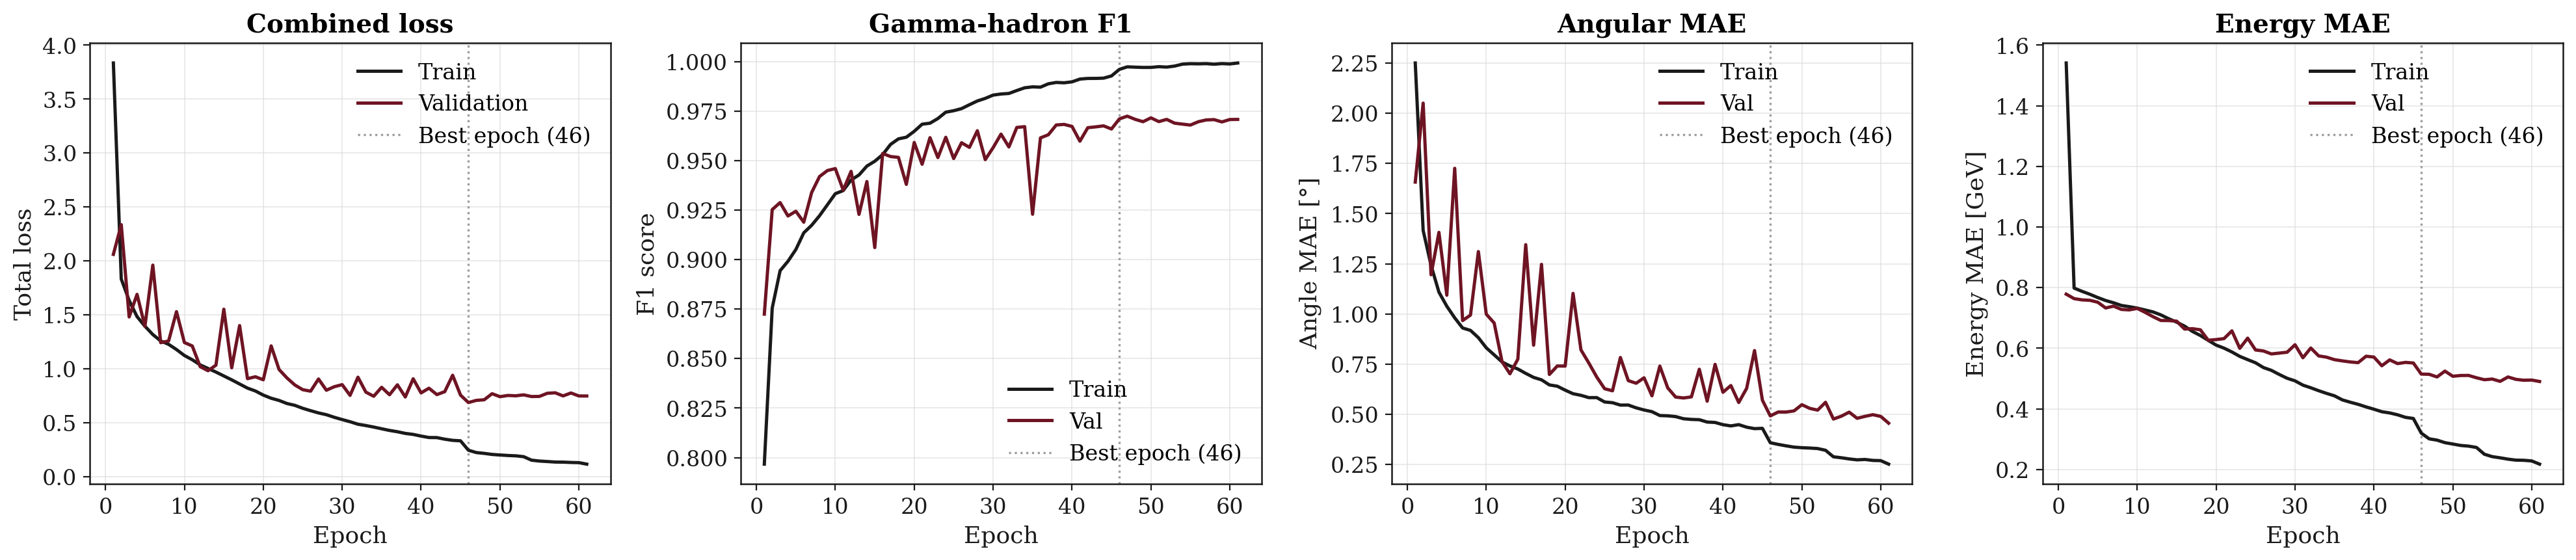
\includegraphics[width=1\linewidth]{figures/training_curves.png}
    \caption[Training and validation curves across the three tasks.]{Training and validation curves as a function of epoch. From left to right: combined multi-task loss, gamma-hadron F1 score, angular MAE, and energy MAE. The vertical dotted line in each panel marks the best checkpoint epoch (minimum combined validation loss), restored for the final evaluation. All tasks converge jointly without divergence.}
    \label{fig:training_curves}
\end{figure*}

A note on notation is in order before the results are presented. Throughout this chapter, a circumflex denotes a quantity predicted by the model and the subscript ``true'' denotes the corresponding Monte Carlo value: $\hat{\theta}$ and $\theta_\text{true}$ are the reconstructed and true zenith angles of an event, and $\hat{E}$ and $E_\text{true}$ its reconstructed and true primary energies. The \textit{angular residual} of an event is the difference $\hat{\theta} - \theta_\text{true}$, and its absolute value $|\hat{\theta} - \theta_\text{true}|$ is the absolute angular error.

Table~\ref{tab:performance_summary} provides a consolidated view of the primary metrics across all three tasks, including domain-specific figures of merit.

\begin{table}[ht!]
\centering
\caption[Summary of multi-task reconstruction performance.]{Summary of multi-task reconstruction performance on the test set, including domain-specific figures of merit. $Q = \varepsilon_\gamma / \sqrt{\varepsilon_p}$ is the quality factor for gamma-hadron separation, defined in full in Section~\ref{sec:apx_qfactor}. PSF$_{68}$ is the 68\% containment radius of the angular residual distribution, defined in full in Section~\ref{sec:apx_psf}.}
\label{tab:performance_summary}
\setlength{\tabcolsep}{8pt}
\renewcommand{\arraystretch}{1.2}
\begin{tabular}{lll}
\toprule
\textbf{Task} & \textbf{Primary Metric} & \textbf{Additional} \\
\midrule
Gamma-Hadron   & AUC = 0.991      & $Q$-factor = 5.48, $\varepsilon_\gamma = 0.971$ \\
Zenith Angle   & MAE = $0.484\degree$ & PSF$_{68}$ = $0.50\degree$, RMS = $0.74\degree$ \\
Energy         & MAE = 103.72 GeV & $\sigma_E / E$ = 33.1\%, $R^2$ = 0.453 \\
\bottomrule
\end{tabular}
\end{table}

\subsection{Gamma-Hadron Discrimination}
\label{subsec:particle}

Table~\ref{tab:particle_metrics} summarizes the classification performance on the test set. The model achieves an area under the receiver operating characteristic (ROC) curve (AUC) of 0.991, an F1-score of 0.970, and an overall accuracy of 96.99\%. The quality factor $Q = \varepsilon_\gamma / \sqrt{\varepsilon_p}$, a standard figure of merit in gamma-ray astronomy that quantifies signal-to-noise ratio, evaluates to $Q = 5.48$.

\begin{table}[ht!]
\centering
\caption[Gamma-hadron discrimination performance on the test set.]{Classification performance on the test set. Precision, recall, and F1-score are reported for each class. The test partition comprises 11,209 events, 5,606 proton-induced and 5,603 gamma-induced, so the two classes are balanced to within 0.03\%.}
\label{tab:particle_metrics}
\setlength{\tabcolsep}{9pt}
\renewcommand{\arraystretch}{1.15}
\begin{tabular}{lccc}
\toprule
\textbf{Class} & \textbf{Precision} & \textbf{Recall} & \textbf{F1} \\
\midrule
Proton   & 0.971 & 0.969 & 0.970 \\
$\gamma$ & 0.969 & 0.971 & 0.970 \\
\midrule
\textbf{Overall} & \multicolumn{3}{c}{Accuracy: \textbf{96.99\%} $\quad$ AUC: \textbf{0.991}} \\
\bottomrule
\end{tabular}
\end{table}

Figure~\ref{fig:particle_results} shows the row-normalized confusion matrix, with the raw event counts, and the ROC curve. Both classes are reconstructed with high fidelity: $96.9\%$ of proton events and $97.1\%$ of gamma events are classified correctly, and the ROC curve rises steeply to an AUC of $0.991$. The few percent of misclassified events correspond to the small overlap between the two classes near the decision threshold at $P(\gamma)=0.5$.

\begin{figure*}[ht!]
    \centering
    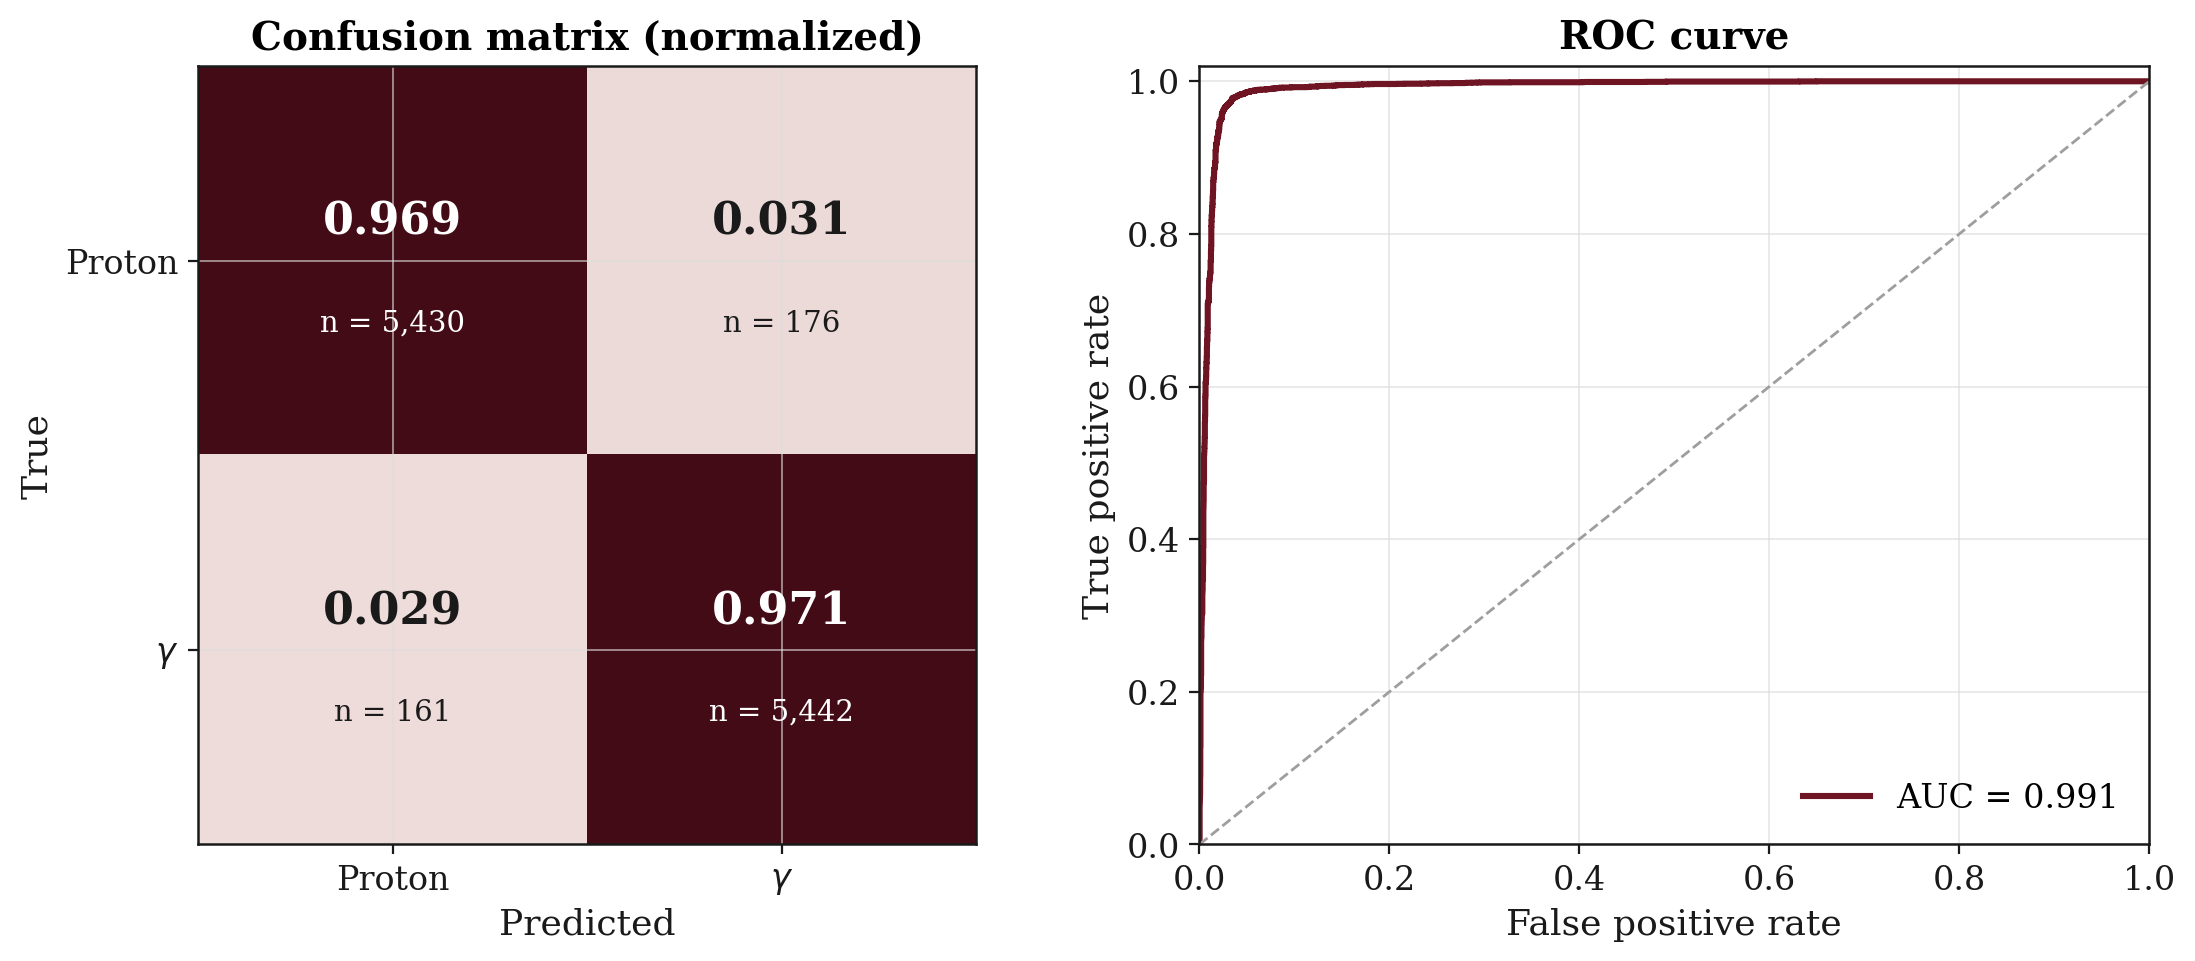
\includegraphics[width=1\linewidth]{figures/particle_results.png}
    \caption[Gamma-hadron discrimination results.]{Gamma-hadron discrimination on the test set. \textbf{Left:} row-normalized confusion matrix, with the raw event count shown below each fraction. \textbf{Right:} ROC curve (AUC = 0.991).}
    \label{fig:particle_results}
\end{figure*}

Figure~\ref{fig:roc_stratified} shows the ROC curves grouped by primary energy and by zenith angle bin: each curve is computed separately within the events sharing a given value of that variable, rather than over the test set as a whole, which isolates how discrimination depends on it. Discrimination improves at lower energies: the AUC is 0.998 at 300 GeV, 0.991 at 500 GeV, and 0.981 at 800 GeV.

This trend is physically consistent. At 300 GeV, electromagnetic showers are compact with a well-defined core signature, while hadronic showers at the same energy are sparse and noisy, making the morphological contrast between the two classes large. As the primary energy increases toward 800 GeV, both shower types develop larger and more complex footprints with greater stochastic fluctuations. In addition, a growing fraction of the energy of a hadronic shower is channelled into its electromagnetic component through neutral pion decay, the mechanism described in Section~\ref{subsec:hadronic_showers}. Hadronic events therefore acquire progressively more of the compact, centrally concentrated signature that distinguishes gamma-induced showers in the first place. Both effects reduce the morphological contrast between the two classes.

Across zenith angle bins the AUC ranges from 0.984 to 0.994, so discrimination is essentially independent of shower inclination over the range covered by the training data.

\begin{figure}[ht!]
    \centering
    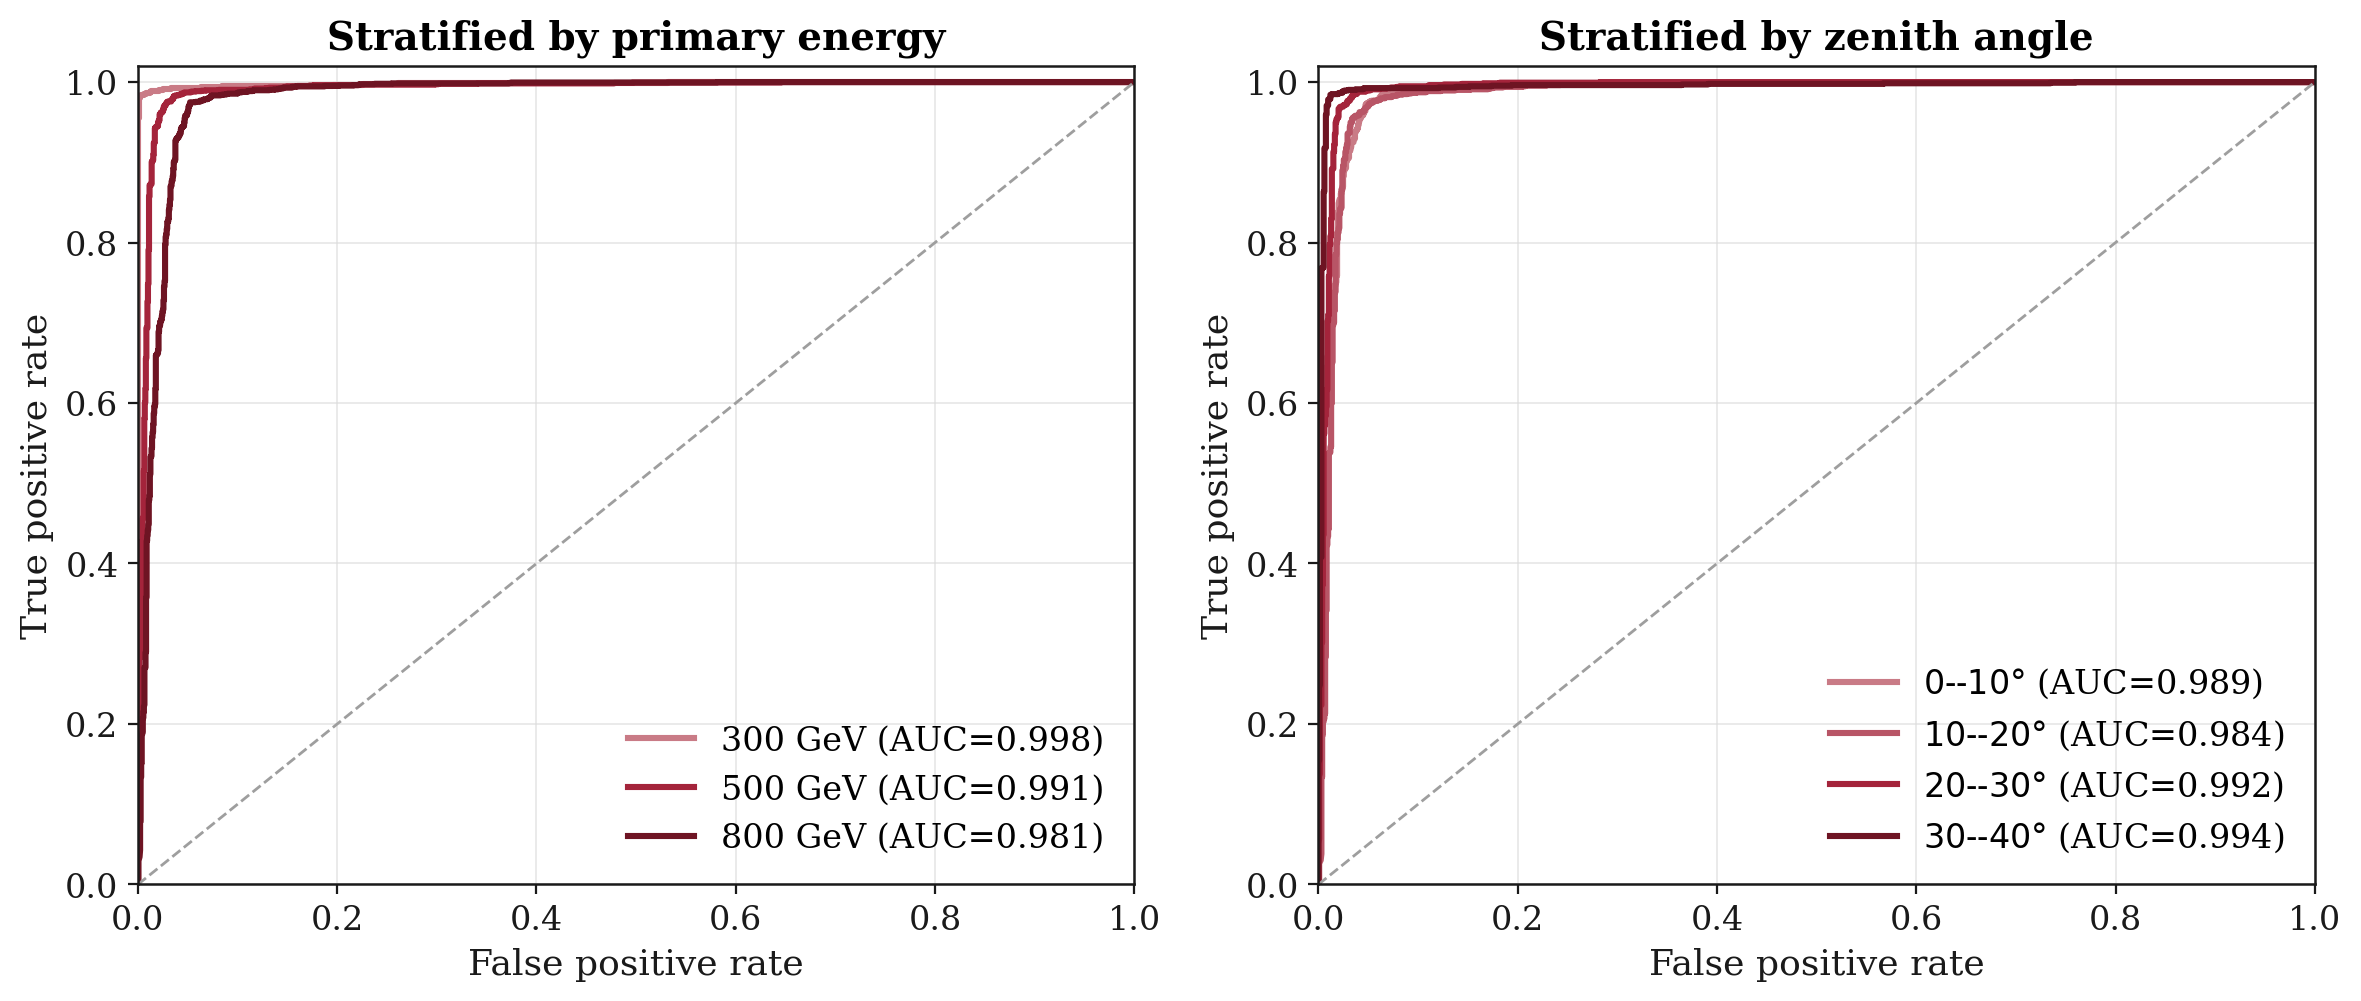
\includegraphics[width=0.85\linewidth]{figures/roc_stratified.png}
    \caption[ROC curves grouped by energy and zenith angle.]{ROC curves for gamma-hadron discrimination, grouped by primary energy (left) and zenith angle bin (right). AUC values are shown in the legend for each group.}
    \label{fig:roc_stratified}
\end{figure}

\subsection{Zenith Angle Reconstruction}
\label{subsec:angle}

The model achieves a mean absolute error of $\text{MAE}_\theta = 0.484\degree$ on the test set, with a coefficient of determination $R^2 = 0.996$. These results represent a significant improvement over both the traditional reconstruction baseline for CONDOR reported in~\shortciteA{arratia2025condor} (approximately 1--2\degree) and the predecessor CNN-LSTM model of~\shortciteA{navarro2025multi} ($\text{MAE}_\theta = 1.14\degree$). Table~\ref{tab:angle_metrics} summarizes the angular resolution metrics.

\begin{table}[ht!]
\centering
\caption[Zenith angle reconstruction metrics on the test set.]{Zenith angle reconstruction performance on the test set.}
\label{tab:angle_metrics}
\setlength{\tabcolsep}{11pt}
\renewcommand{\arraystretch}{1.15}
\begin{tabular}{lc}
\toprule
\textbf{Metric} & \textbf{Value} \\
\midrule
MAE            & $0.484\degree$ \\
RMSE           & $0.736\degree$ \\
$R^2$          & 0.996 \\
\bottomrule
\end{tabular}
\end{table}

Figure~\ref{fig:angle_results} shows the absolute and relative error distributions by particle type, together with the linearity profile $\mathbb{E}[\hat{\theta}\,|\,\theta_\text{true}]$. The absolute error distribution is heavily concentrated below $1\degree$ for both particle types, with a mean bias of $+0.036\degree$, confirming that the model is nearly unbiased across the range. Events with $\theta_\text{true} = 0\degree$ are excluded from the relative error panel, as the fractional residual $(\hat{\theta} - \theta_\text{true})/\theta_\text{true}$ is undefined at the origin. The linearity profile follows the ideal diagonal closely, with residuals that are symmetric and stable from $0\degree$ to $40\degree$.

\begin{figure*}[ht!]
    \centering
    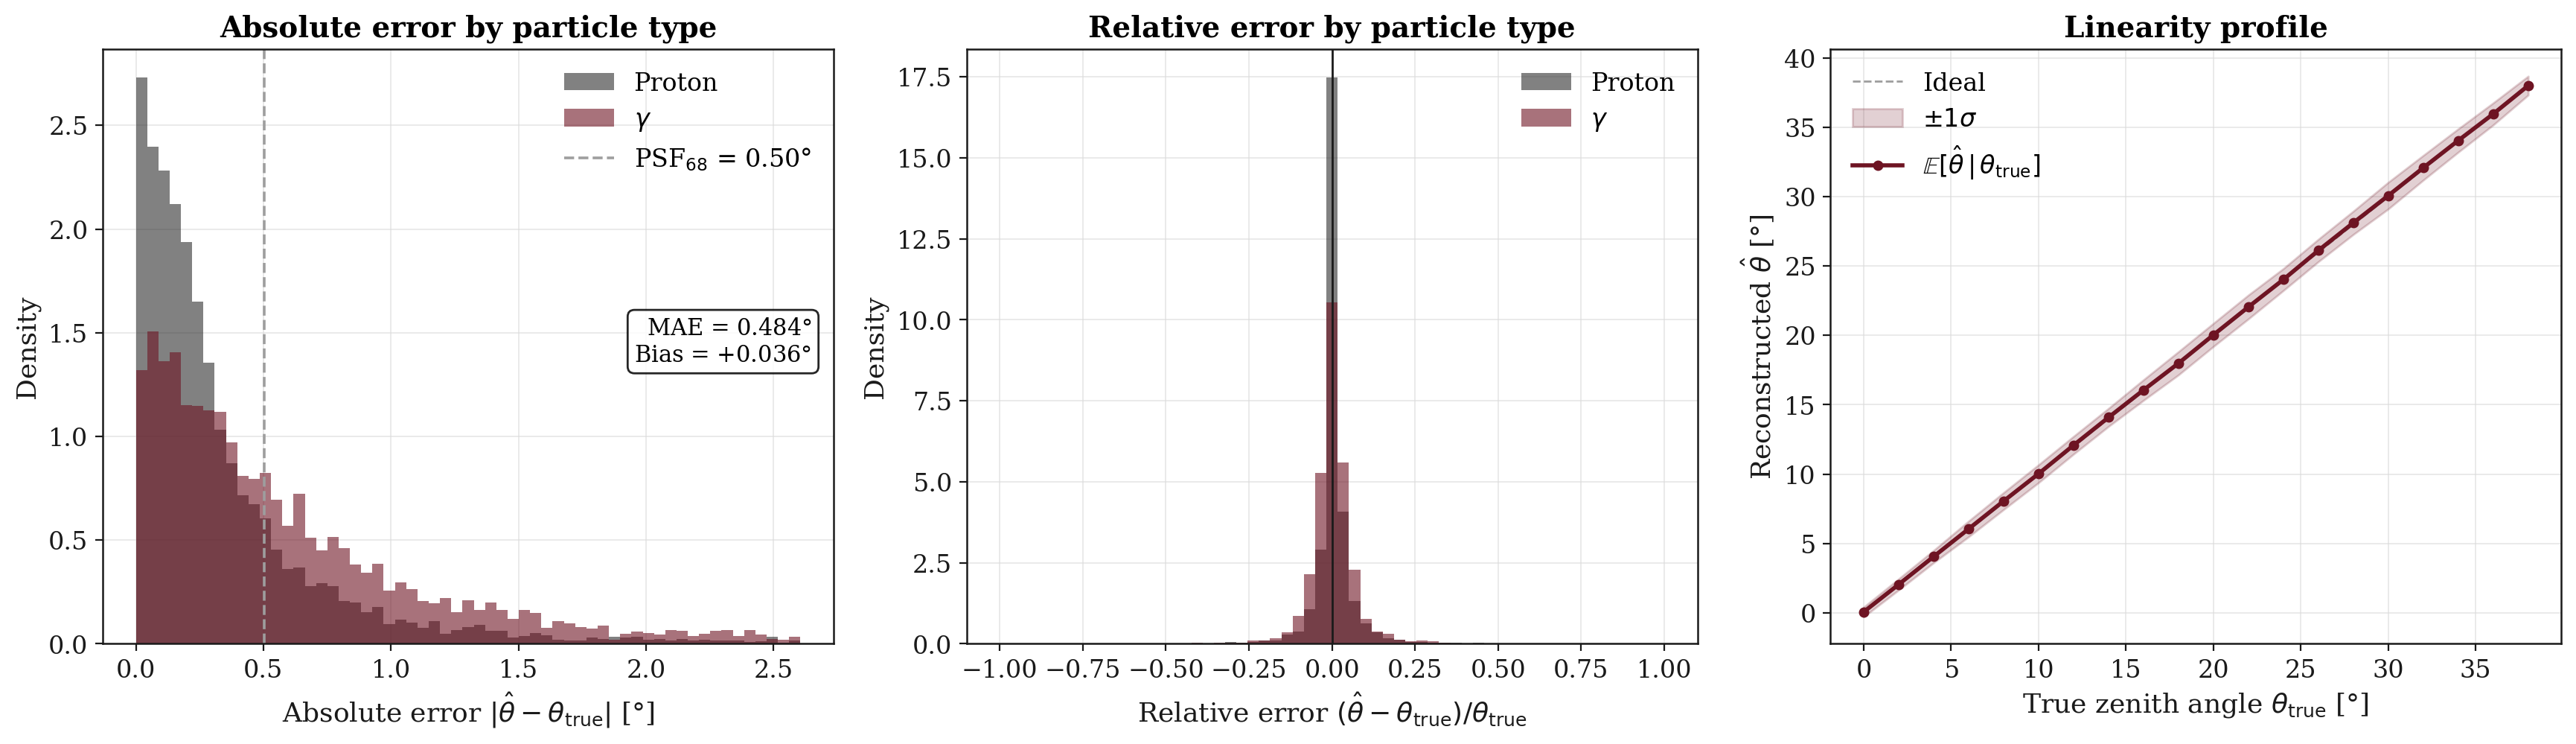
\includegraphics[width=1\linewidth]{figures/angle_results.png}
    \caption[Zenith angle reconstruction results.]{Zenith angle reconstruction on the test set. \textbf{Left:} distribution of the absolute error $|\hat{\theta}-\theta_\text{true}|$ for proton and gamma events, with key metrics inset. \textbf{Center:} relative error distribution $(\hat{\theta}-\theta_\text{true})/\theta_\text{true}$ by particle type. \textbf{Right:} mean reconstructed angle $\mathbb{E}[\hat{\theta}\,|\,\theta_\text{true}]$ with $\pm 1\sigma$ bands, confirming linearity across the full $0\degree$--$40\degree$ range.}
    \label{fig:angle_results}
\end{figure*}

The MAE of $0.484\degree$ corresponds to sub-degree pointing accuracy. The 68\% containment radius of the angular residual distribution, PSF$_{68} = 0.50\degree$, is the standard figure of merit for source identification in gamma-ray astronomy. The RMSE-to-MAE ratio of 1.52 is moderately above the value expected for a pure Gaussian residual distribution ($\sqrt{\pi/2} \approx 1.25$), indicating mildly heavier-than-Gaussian tails; large outlier reconstructions are present but infrequent. Performance is stable across the full $0\degree$--$40\degree$ zenith range covered by the training data.

\subsection{Energy Estimation}
\label{subsec:energy}

Energy estimation is the most challenging of the three tasks due to the discrete and narrow primary energy range (300--800 GeV). The model achieves $\text{MAE}_E = 103.72$ GeV and $\text{RMSE}_E = 151.80$ GeV on the test set, with an overall fractional energy resolution $\sigma_E/E = 33.1\%$ and $R^2 = 0.453$. The stratified analysis in Table~\ref{tab:energy_stratified} shows that the resolution varies substantially by particle type and energy, ranging from 16--20\% for protons across all energy bins to 45\% for gamma events at 300 GeV. The low $R^2$ reflects the discrete nature of the three training energies rather than a modeling failure: the coefficient of determination penalizes the large inter-class variance that dominates when only three energy values are present. Table~\ref{tab:energy_metrics} summarizes the scalar metrics.

\begin{table}[ht!]
\centering
\caption[Energy estimation metrics on the test set.]{Energy estimation performance on the test set.}
\label{tab:energy_metrics}
\setlength{\tabcolsep}{11pt}
\renewcommand{\arraystretch}{1.15}
\begin{tabular}{lc}
\toprule
\textbf{Metric} & \textbf{Value} \\
\midrule
MAE  & 103.72 GeV \\
RMSE & 151.80 GeV \\
Pull $\sigma$ & 0.331 \\
\bottomrule
\end{tabular}
\end{table}

The bias analysis reveals a systematic energy-dependent trend, summarized in Table~\ref{tab:energy_stratified}: the model overestimates at 300 GeV and underestimates at 800 GeV, with the effect more pronounced for gamma events than for protons. This is a consequence of the discrete training energies combined with shower fluctuations. At 300 GeV, electromagnetic showers can occasionally develop late, producing a footprint more typical of a higher-energy event; at 800 GeV, shower fluctuations in the opposite direction cause the model to pull predictions toward the center of the energy range. This regression-toward-the-mean bias is expected for discrete-target regression and should be accounted for when applying the model to analysis pipelines.

\begin{table}[ht!]
\centering
\caption[Energy bias and resolution split by particle type.]{Energy bias and resolution per true energy bin, split by particle type. Bias = mean fractional deviation $(\hat{E}-E)/E$; Resolution = standard deviation of the fractional residual. Both expressed as percentages.}
\label{tab:energy_stratified}
\setlength{\tabcolsep}{8pt}
\renewcommand{\arraystretch}{1.2}
\begin{tabular}{lccccc}
\toprule
 & \multicolumn{2}{c}{\textbf{Proton}} & & \multicolumn{2}{c}{\textbf{Gamma}} \\
\cmidrule{2-3} \cmidrule{5-6}
\textbf{Energy} & Bias (\%) & Res. (\%) & & Bias (\%) & Res. (\%) \\
\midrule
300 GeV & $+6.0$  & 20.2 & & $+43.8$ & 45.3 \\
500 GeV & $+6.0$  & 19.9 & & $+12.0$ & 29.2 \\
800 GeV & $-11.2$ & 15.5 & & $-17.7$ & 17.5 \\
\bottomrule
\end{tabular}
\end{table}

Figure~\ref{fig:energy_analysis} shows the overall pull distribution and its decomposition by particle type. The overall pull is approximately Gaussian with $\mu = 0.065$ and $\sigma = 0.331$; the small positive mean indicates a systematic overestimation of approximately $6.5\%$, consistent with the regression-toward-the-mean effect identified in the stratified analysis: the model pulls extreme predictions toward the center of the training energy range. The per-class pull distributions confirm the same class asymmetry visible in Table~\ref{tab:energy_stratified}: proton events have a substantially narrower pull ($\sigma_p \approx 0.20$) than gamma events ($\sigma_\gamma \approx 0.41$). Proton-induced showers spread over many detectors with a stable lateral profile at fixed energy, whereas gamma-induced showers depend more sensitively on the electromagnetic-core position within the array, which is a larger source of variance for energy inference. Proton events are essentially unbiased ($\mu_p \approx 0.004$), while the overall positive mean of the combined distribution is driven primarily by a $\sim 13\%$ overestimate in the gamma class ($\mu_\gamma \approx 0.13$).

\begin{figure*}[ht!]
    \centering
    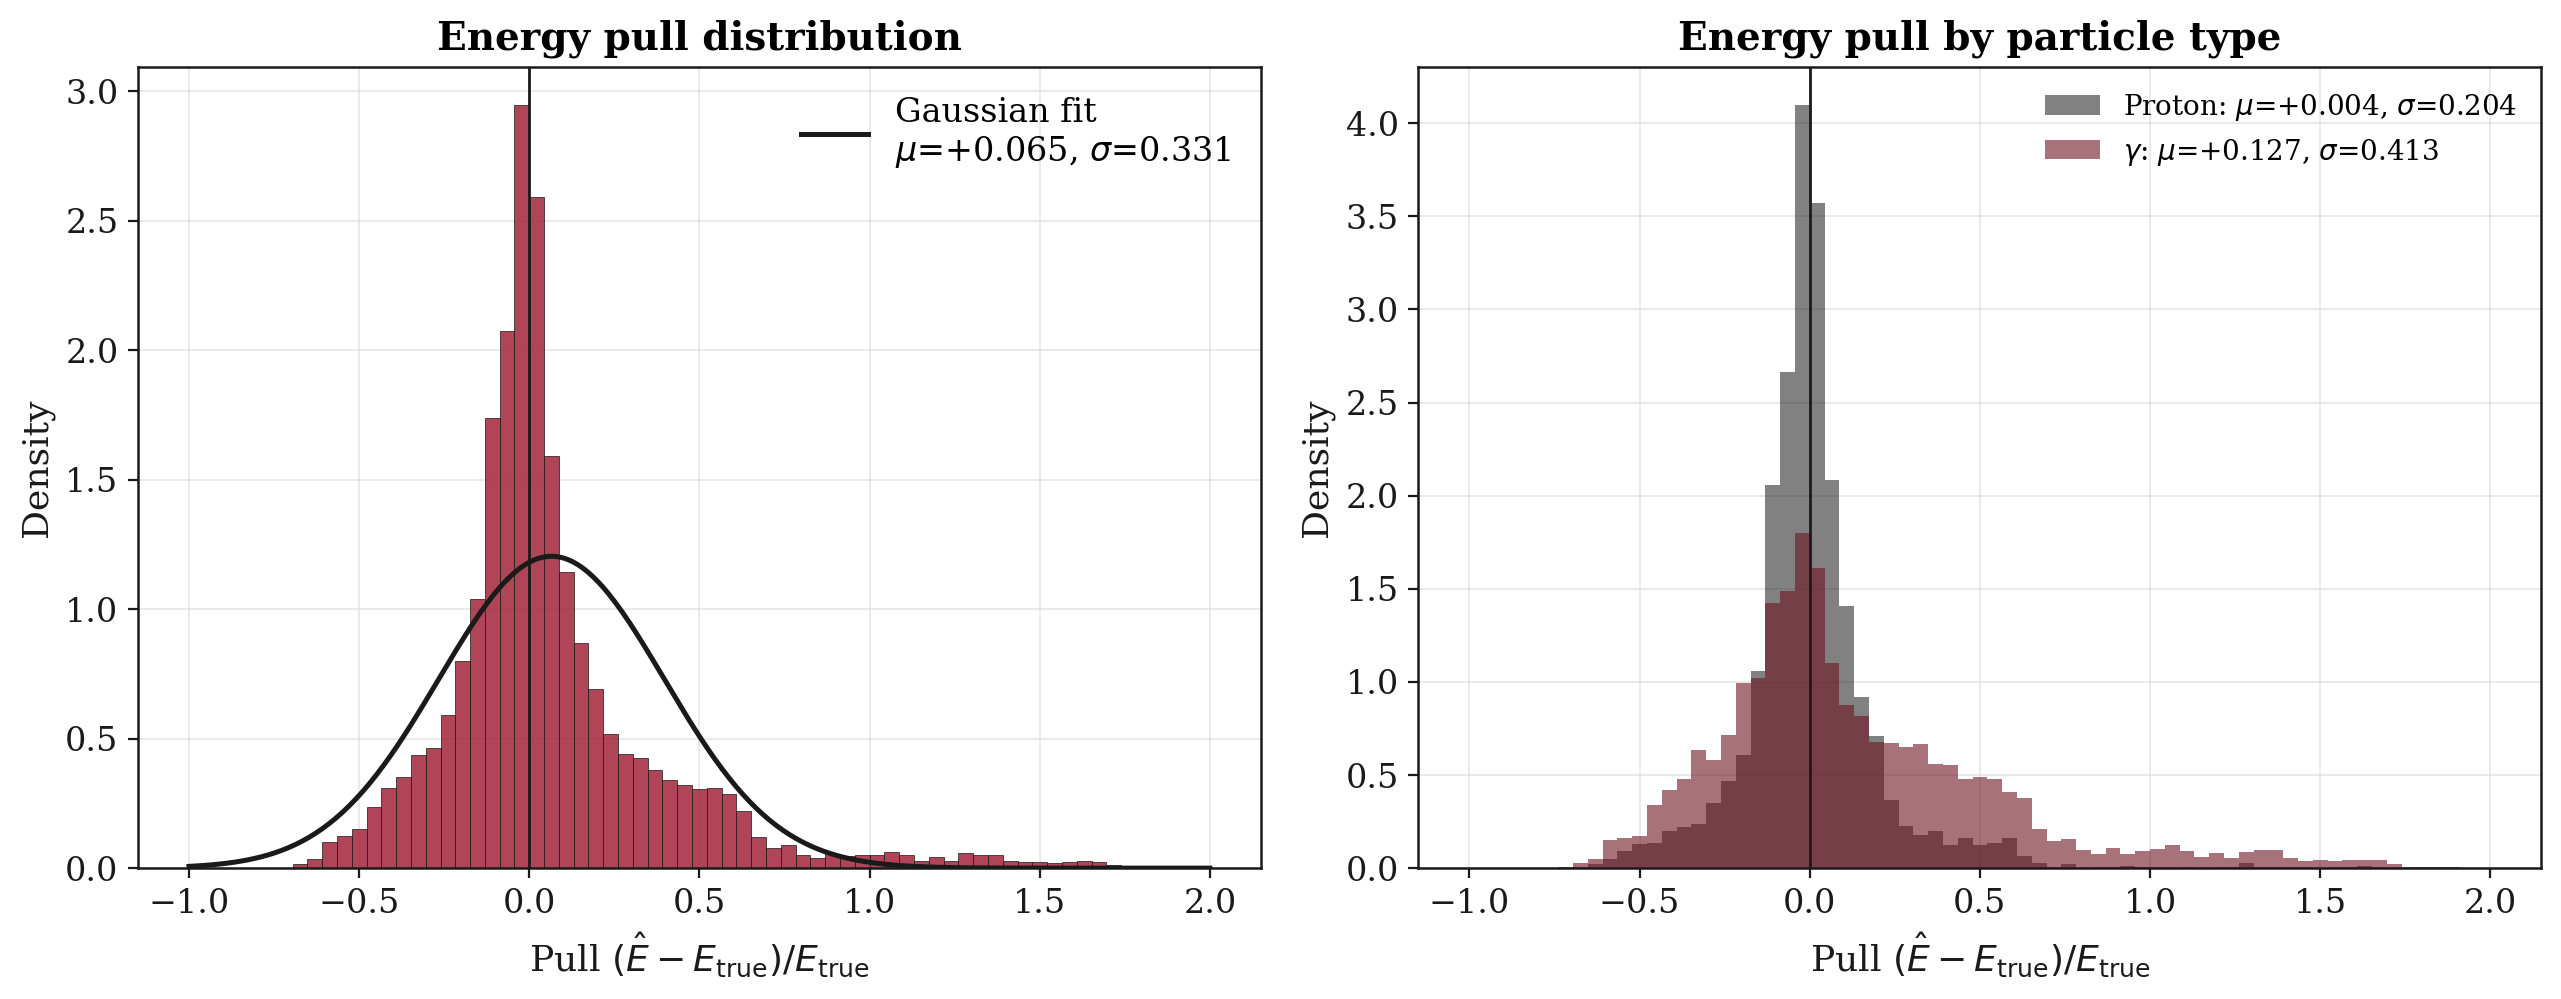
\includegraphics[width=1\linewidth]{figures/energy_analysis.png}
    \caption[Energy pull distribution overall and by particle type.]{Energy estimation analysis. \textbf{Left:} overall pull distribution $(\hat{E} - E_\mathrm{true})/E_\mathrm{true}$ with Gaussian reference curve ($\mu = 0.065$, $\sigma = 0.331$). \textbf{Right:} pull distribution split by particle type; both classes are essentially unbiased but gamma events show roughly twice the width of proton events, consistent with the per-class resolutions in Table~\ref{tab:energy_stratified}.}
    \label{fig:energy_analysis}
\end{figure*}

The energy head produces a continuous estimate, so a rule is required to place each prediction into one of the three energy bins of the dataset. Each event is assigned to the bin whose nominal energy is closest to its prediction, that is, to the value in $\{300, 500, 800\}$~GeV minimizing $|\hat{E} - E_\text{bin}|$. This is equivalent to cutting the continuous axis at the midpoints between consecutive levels, at 400 and 650 GeV. The assignment is used only to build the matrix and plays no part in training or in any of the regression metrics reported above, all of which are computed on the continuous predictions.

Figure~\ref{fig:migration_matrix} shows the resulting energy migration matrix, which reports for each true energy bin the fraction of events reconstructed in each of the three energy bins. The diagonal elements are 75.0\%, 68.2\%, and 67.5\% for 300, 500, and 800 GeV respectively. The largest off-diagonal entry is the 27.8\% migration from 800 GeV to the 500 GeV bin: more than a quarter of high-energy events are systematically reconstructed at a lower energy. This is consistent with the negative bias at 800 GeV identified above and reflects the inherent difficulty of separating 500 and 800 GeV showers in the sub-TeV regime, where the difference in shower size and footprint between adjacent energy bands can be within the natural fluctuation range of individual events.

\begin{figure}[ht!]
    \centering
    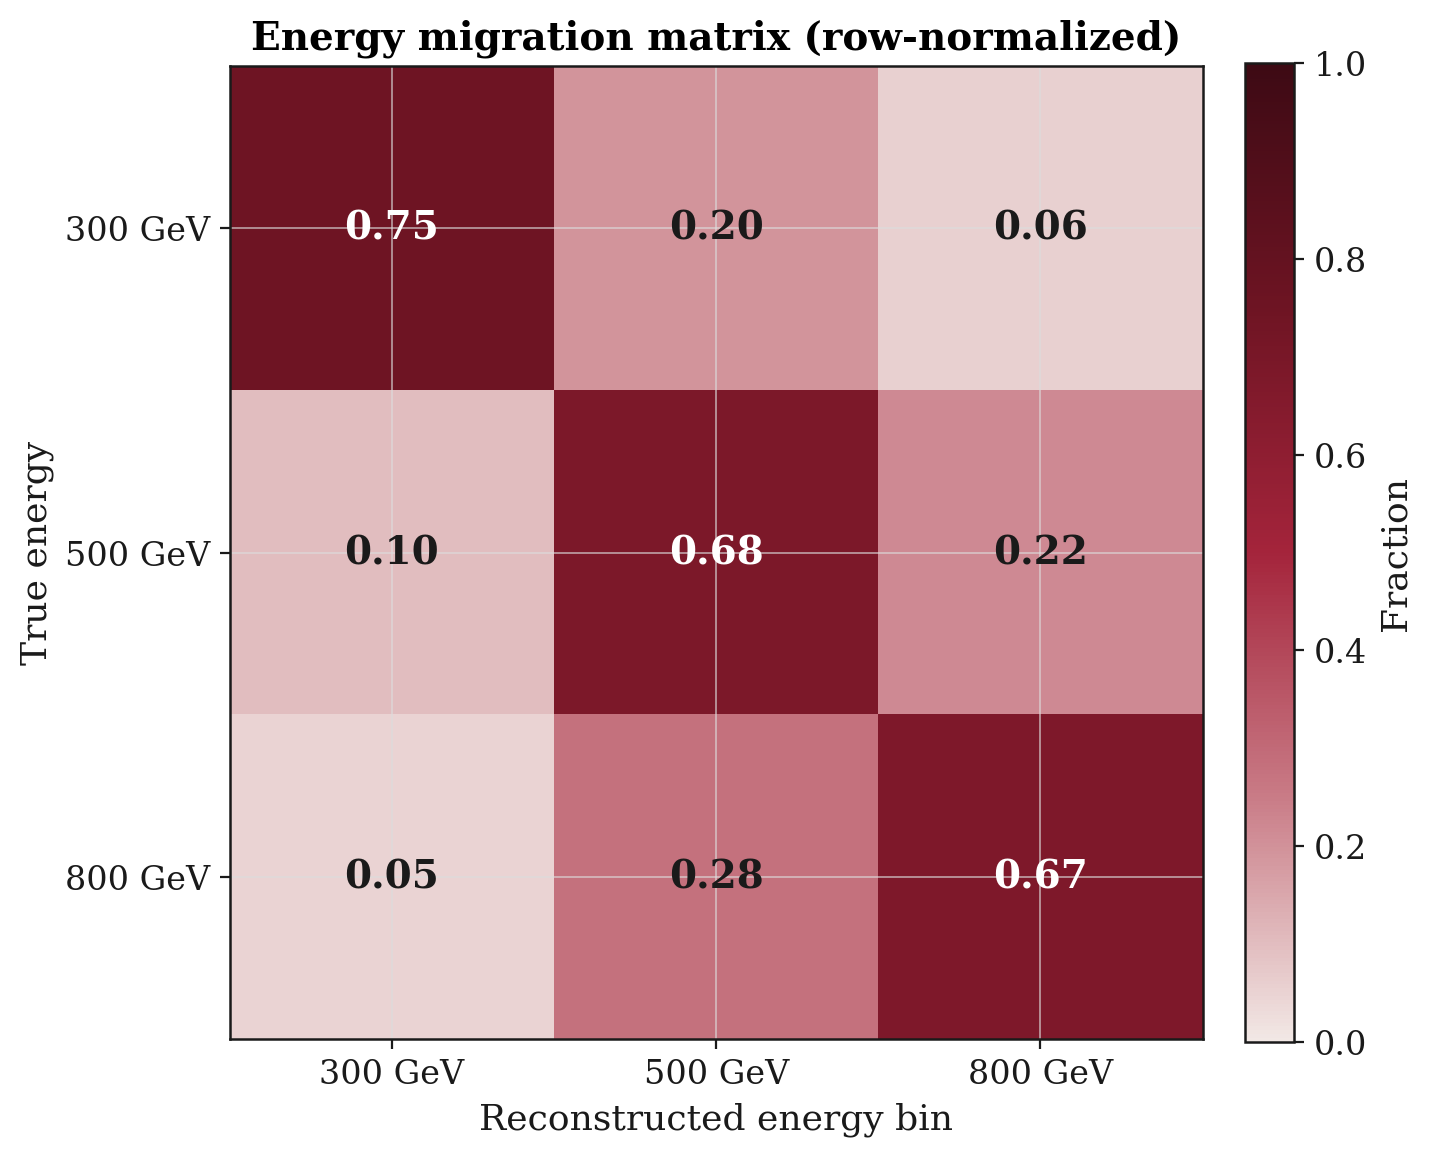
\includegraphics[width=0.62\linewidth]{figures/energy_migration_matrix.png}
    \caption[Energy migration matrix.]{Energy migration matrix. Each row gives the fraction of events at a given true energy that are reconstructed in each of the three energy bins (row-normalized). A dominant diagonal indicates low migration; off-diagonal entries indicate systematic misreconstruction between adjacent energy bins.}
    \label{fig:migration_matrix}
\end{figure}

\subsection{Comparison with the State of the Art}
\label{subsec:sota}

Table~\ref{tab:sota} places the results in the context of prior work on deep learning for EAS reconstruction. Direct comparisons across experiments are complicated by differences in detector technology, altitude, energy range, and the number of simultaneously reconstructed quantities; the table therefore includes the relevant context for each comparison. The model presented in this thesis is the only published work to address three reconstruction tasks simultaneously, at this altitude and energy range, with an integrated explainability framework.

\begin{table}[ht!]
\centering
\caption[Comparison with state-of-the-art EAS reconstruction.]{Comparison with selected published results on deep learning for EAS reconstruction. \textit{Tasks}: number of simultaneously reconstructed quantities (g/h = gamma-hadron, $\theta$ = zenith angle, $E$ = energy). Dashes indicate metrics not reported or not applicable.}
\label{tab:sota}
\renewcommand{\arraystretch}{1.2}
\resizebox{\linewidth}{!}{%
\begin{tabular}{llcclcc}
\toprule
\textbf{Reference} & \textbf{Observatory} & \textbf{Alt.} & \textbf{Energy range} & \textbf{Tasks} & \textbf{g/h AUC} & \textbf{Ang.\ MAE} \\
\midrule
This work & CONDOR & 5,300 m & 300--800 GeV & 3 (g/h, $\theta$, $E$) & \textbf{0.991} & $\mathbf{0.484\degree}$ \\
\shortciteA{navarro2025multi} & CONDOR & 5,300 m & 150--800 GeV & 2 (g/h, $\theta$) & F1=0.89 & $1.14\degree$ \\
\shortciteA{arratia2025condor} & CONDOR & 5,300 m & 100 GeV--1 TeV & $\theta$ & --- & $1$--$2\degree$ \\
\shortciteA{okukawa2024neural} & Tibet AS$\gamma$ & 4,300 m & 10--100 TeV & 1 (g/h) & 0.781--0.901 & --- \\
\shortciteA{erdmann2018deep} & Pierre Auger & 1,400 m & 3--100 EeV & 1 ($\theta$) & --- & $1.2\degree$ \\
\bottomrule
\end{tabular}}
\end{table}

The methods and published results against which this work is compared are described in Section~\ref{sec:related_work}. The angular resolution of $0.484\degree$ represents a factor of 2.4 improvement over the predecessor model~\shortciteA{navarro2025multi} and places the reconstruction well below the 1\degree~threshold typically required for point-source identification in gamma-ray astronomy. The gamma-hadron AUC of 0.991 is achieved at a substantially lower energy range and with a more complex multi-task constraint than the comparable scintillator-array results of~\shortciteA{okukawa2024neural}, who report AUC values of 0.781--0.901 at 10--100 TeV on a single-task network. The most directly comparable gamma-hadron study in our energy window is that of~\shortciteA{conceiccao2025discriminating}, who apply a pretrained vision transformer to the shower footprint of a water-Cherenkov array at 5{,}200~m over the 200~GeV--1~TeV range, reporting a proton rejection of approximately 97\% at a gamma efficiency of 80\%. 

A direct AUC comparison with their work is not possible because they quote performance at fixed efficiency working points rather than a threshold-integrated metric, and their detector technology (water Cherenkov) differs from the CONDOR scintillator array; nonetheless, their results corroborate that sub-TeV footprint morphology carries strong discriminating power. Energy estimation, by contrast, is not directly comparable across experiments, as the energy ranges and figures of merit differ substantially: \shortciteA{meng2025machine}, for instance, reconstruct primary energy for Tibet AS$\gamma$ but over the 1~TeV--10~PeV range, where the resolution behaves intrinsically differently. The migration matrix in Figure~\ref{fig:migration_matrix} therefore provides the most informative characterization of energy reconstruction quality for this work.

% ============================================================
\section{Explainability Analysis}
\label{sec:explainability}
% ============================================================

Two complementary feature importance methods --- a feature ablation study and permutation feature importance --- are applied to validate that the learned representations are physically consistent. Because both quantify the same notion (the degradation in task performance when a single input feature is disabled) and yield mutually consistent rankings, they are presented together. They are followed by an analysis of the attention patterns extracted from the RAW Transformer streams, which provide hit-level interpretability directly in the space of detector observables.

\subsection{Feature Importance}
\label{subsec:feature_importance}

The term \emph{ablation} is borrowed from experimental neuroscience, where lesion studies selectively remove or disable a region of the brain and infer the function of that region from the behavioural deficit that follows; the same methodology was later adopted to probe the internal representations of artificial neural networks~\shortciteA{meyes2019ablation}. The \textbf{feature ablation study} applies this logic at the level of the input: it measures the importance of each input feature by replacing it with its median value across the training set --- computed over non-padded positions only --- and evaluating the resulting degradation in test-set performance, attributing the loss to the information that the disabled feature carried.

\textbf{Permutation feature importance} (PFI)~\shortciteA{altmann2010permutation} instead randomly permutes a single feature across all test-set events, breaking its correlation with the target while preserving its marginal distribution. The two are complementary: ablation collapses a feature to a single typical value and is therefore sensitive to the loss of its typical variation, whereas PFI preserves the full distribution and is more sensitive to the information carried by a feature's extreme values. Both methods are applied independently to each of the six sequential features --- \texttt{detector\_id}, \texttt{particle\_count}, \texttt{t\_bin}, \texttt{total\_energy}, \texttt{x\_center}, and \texttt{y\_center} --- for each of the three tasks. Figures~\ref{fig:ablation} and~\ref{fig:pfi} report the relative degradation, expressed as a percentage of the baseline metric, for ablation and PFI respectively.

\textbf{Zenith angle.} Both methods agree that \texttt{t\_bin} is by far the most important feature for angular reconstruction. Ablation increases the MAE from its baseline of $0.484\degree$ to $12.9\degree$ (a relative degradation of approximately 2{,}568\%), and PFI yields a comparable $\Delta\text{MAE} = 12.76\degree$. This is physically expected: the arrival time of each detector hit encodes the position of the shower wavefront, and the gradient of arrival times across the array is the primary observable from which the zenith angle is geometrically determined. The next most important features are the spatial coordinates \texttt{x\_center} (ablation $+9.1\degree$, 1{,}889\%; PFI $+5.1\degree$) and \texttt{detector\_id} (ablation $+7.0\degree$, 1{,}456\%; PFI $+3.3\degree$), consistent with the geometric nature of the task.

\textbf{Gamma-hadron discrimination.} For classification both methods place energy deposition and spatial position at the top, with a minor reordering between them. Ablation ranks \texttt{total\_energy} first (accuracy drop of 0.224, a relative degradation of 23.1\%), followed by \texttt{x\_center} (0.136, 14.0\%) and \texttt{t\_bin} (0.118, 12.2\%); PFI ranks \texttt{x\_center} first (0.338, 34.8\%), then \texttt{total\_energy} (0.257, 26.5\%) and \texttt{t\_bin} (0.220, 22.7\%). The prominence of \texttt{total\_energy} reflects the role of the per-hit deposited energy as a tracer of local particle density: electromagnetic showers concentrate this density in a compact core while hadronic showers spread it more widely and irregularly, so the spatial pattern of per-hit energy deposits carries the morphological signature that distinguishes the two classes. The reordering between the two methods reflects the redundancy among the positional features (\texttt{detector\_id}, \texttt{x\_center}, and \texttt{y\_center} all encode hit location): permuting one while leaving the others intact allows partial compensation, distributing the measured importance across the correlated features. Both methods point to a discrimination strategy based on the energy-weighted lateral distribution rather than on single-detector particle identification.

\textbf{Energy estimation.} Spatial position dominates energy reconstruction. Ablation ranks \texttt{x\_center} first ($+106.4$ GeV, 102.6\%), followed by \texttt{detector\_id} ($+83.4$ GeV) and \texttt{t\_bin} ($+72.7$ GeV); PFI ranks \texttt{t\_bin} first ($\Delta\text{MAE} = 173.3$ GeV), followed by \texttt{x\_center} ($143.9$ GeV) and \texttt{detector\_id} ($103.6$ GeV). The spatial position of active hits encodes the shower's lateral extent, which is the strongest predictor of primary energy in ground-based EAS experiments; the prominence of \texttt{t\_bin} under PFI reflects the additional information carried by the full temporal spread of the shower development. Across all three tasks and both methods, \texttt{particle\_count} is the least informative feature (accuracy drop $<0.01$, MAE increase $<1$ GeV), indicating that the number of particles at a given detector adds little beyond what the deposited energy already captures.

\begin{figure*}[ht!]
    \centering
    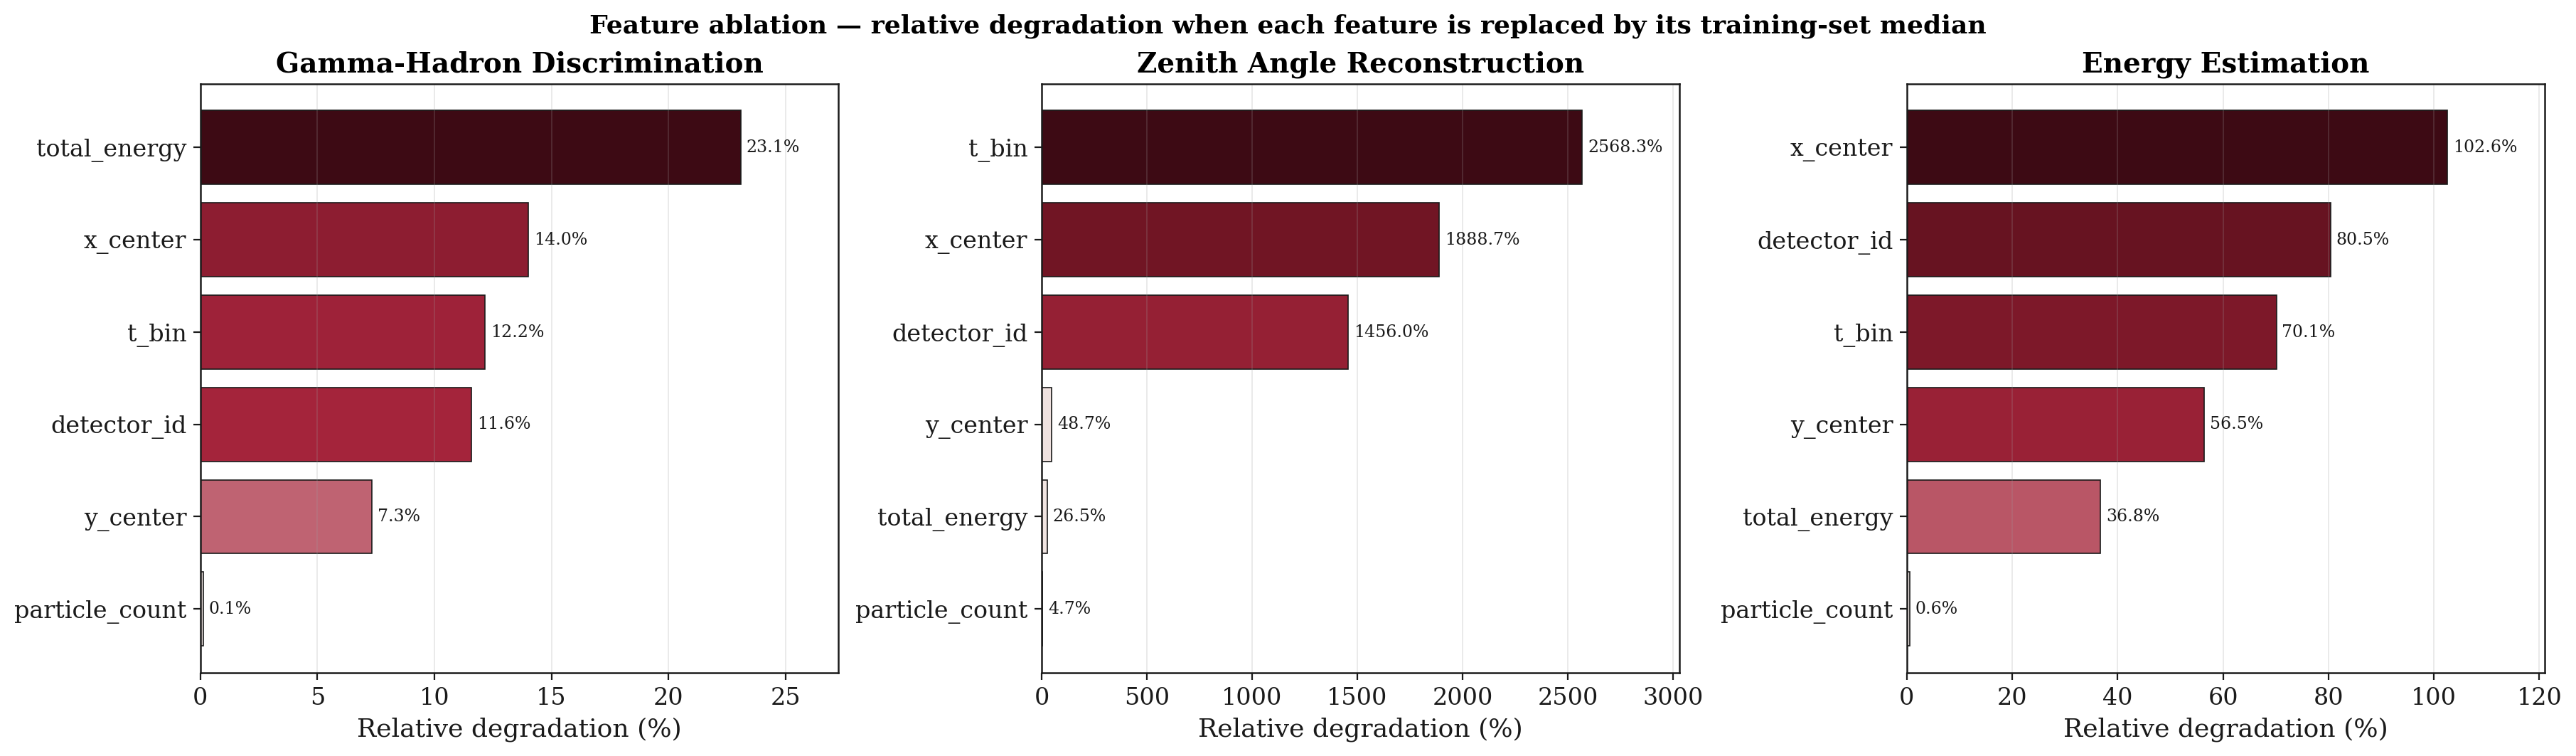
\includegraphics[width=1\linewidth]{figures/feature_ablation.png}
    \caption[Feature ablation study results.]{Feature ablation study: relative degradation, expressed as a percentage of the baseline metric, when each feature is replaced by its training-set median. Each panel corresponds to one reconstruction task; bars are ordered by magnitude and shaded by it.}
    \label{fig:ablation}
\end{figure*}

\begin{figure*}[ht!]
    \centering
    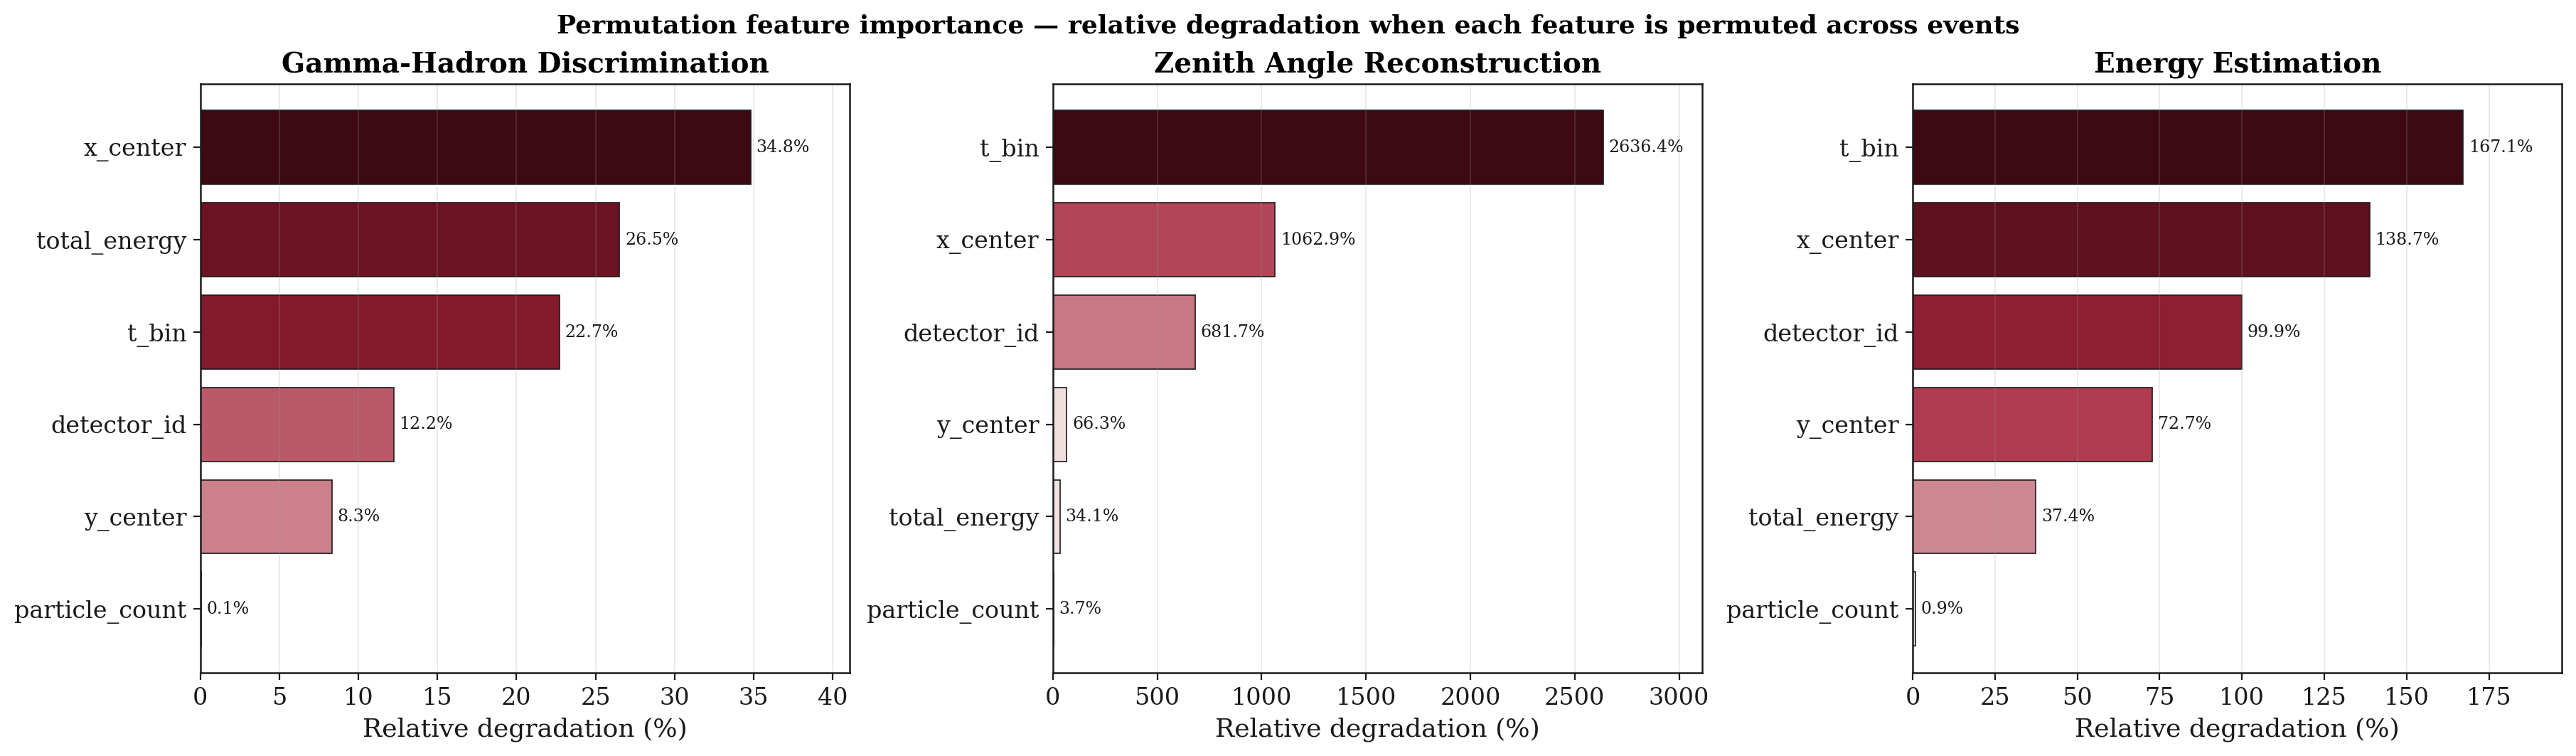
\includegraphics[width=1\linewidth]{figures/pfi_results.png}
    \caption[Permutation feature importance results.]{Permutation feature importance (PFI): relative degradation, expressed as a percentage of the baseline metric, when each feature is permuted across all test-set events. Each panel corresponds to one reconstruction task.}
    \label{fig:pfi}
\end{figure*}

\subsection{Attention Analysis}
\label{subsec:attention}

The RAW Transformer streams operate directly on the masked hit sequence, so their attention weights can be examined at the level of individual detector hits. For an event with $L$ valid hits, $\alpha_{ij}$ denotes the weight that query position $i$ assigns to key position $j$. The weights are produced by a softmax over the valid keys, so that $\sum_{j=1}^{L} \alpha_{ij} = 1$. Two views are reported. The first is the mean attention matrix, averaged over events. The second is the mean attention received by each position,
\begin{equation}
    \bar{\alpha}_{\cdot j} = \frac{1}{L}\sum_{i=1}^{L} \alpha_{ij},
    \label{eq:mean_key_attention}
\end{equation}
which identifies the positions that act as information sources for a stream. Because each row sums to unity, a position of average importance receives a weight of $1/L$; for the mean sequence length of 76.9 valid hits, this reference level is $1.3 \times 10^{-2}$. Hits are ordered chronologically, so low position indices correspond to early-arriving hits, near the leading edge of the shower front. The analysis uses a stratified subsample of 200 test events and the first 120 sequence positions.

\begin{figure*}[ht!]
    \centering
    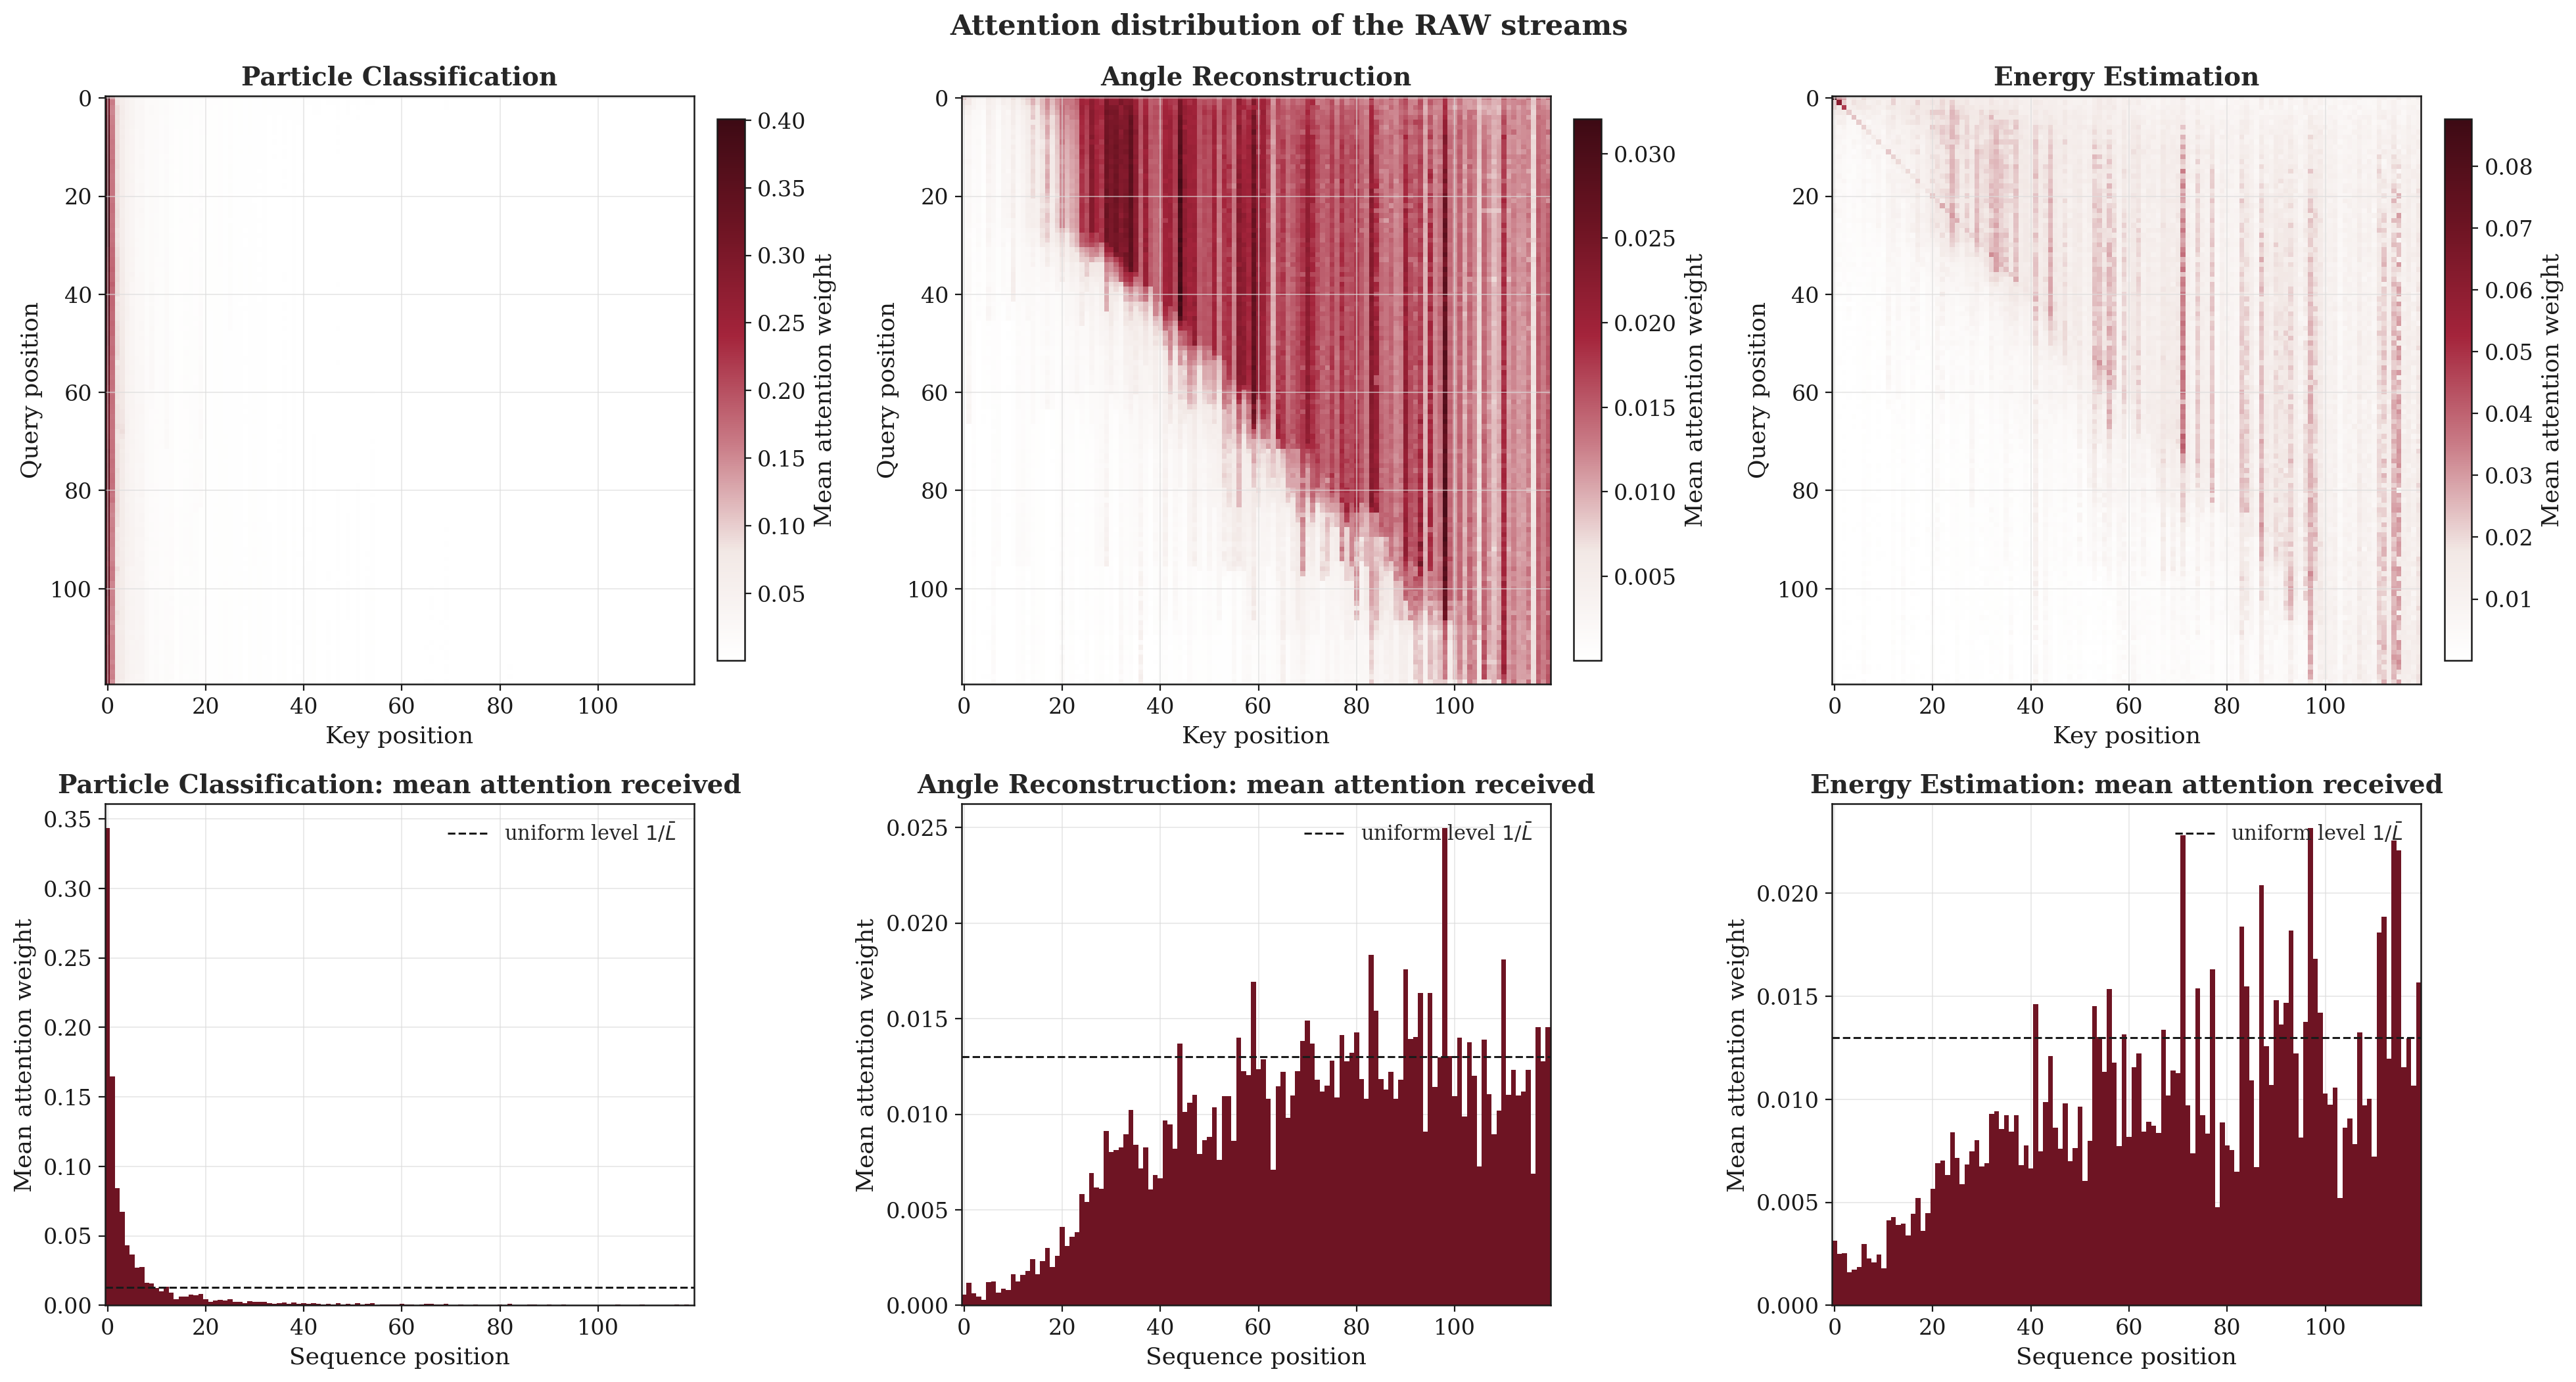
\includegraphics[width=1\linewidth]{figures/attention_patterns_raw.png}
    \caption[Attention distribution of the RAW streams.]{Attention distribution of the three RAW streams. \textbf{Top:} mean attention matrix, averaged over 200 test events; rows are query positions and columns are key positions. \textbf{Bottom:} mean attention received per position, Equation~\eqref{eq:mean_key_attention}; the dashed line marks the uniform reference level $1/\bar{L} = 1.3 \times 10^{-2}$. Cells averaged over fewer than ten events are left blank.}
    \label{fig:attention_patterns}
\end{figure*}

Figure~\ref{fig:attention_patterns} shows both views for the three streams, and the distributions differ markedly between tasks. The classification stream concentrates its weight on the leading edge of the sequence: the first position receives a mean weight of $0.34$, twenty-six times the uniform level, only the first thirteen positions exceed that level, and $82\%$ of the profile lies within the first ten positions. Equivalently, $93\%$ of the matrix weight is assigned to keys that precede the query.

The angle stream shows the opposite ordering. Its profile grows with position, exceeds the uniform level only beyond position 44, and peaks at $2.5 \times 10^{-2}$ near position 98, with $0.7\%$ of the profile in the first ten positions. Correspondingly, $80\%$ of the matrix weight is assigned to keys that follow the query, producing the triangular structure visible in the mean matrix. The energy stream is intermediate: $75\%$ of its weight also falls on later keys, but instead of the smooth ramp of the angle stream the matrix shows isolated bands at specific positions, and a weak diagonal component in which positions attend to their own neighbourhood.

These distributions are consistent with the feature importance results of Section~\ref{subsec:feature_importance}. Zenith angle reconstruction is dominated by \texttt{t\_bin} under both ablation and permutation, and the angle stream accordingly draws its weight from the late part of the sequence, where the arrival-time gradient across the array is defined. Gamma-hadron discrimination depends most strongly on the deposited energy and on the spatial coordinates, quantities that the leading hits already characterize, and the classification stream concentrates on precisely that region. Energy estimation shows the least specialized pattern of the three, which matches its position as the task with the lowest reconstruction quality.

\textbf{Interpretive scope of the attention maps.} Attention weights describe how a stream distributes its reads over the input sequence. They are not an attribution of the prediction to those inputs, and a large weight is not by itself evidence that the corresponding hit was used causally~\shortcite{jain2019attention}. The distributions above are therefore reported as a description of the model's internal weighting, and the feature-level conclusions of this chapter rest on the ablation and permutation analyses of Section~\ref{subsec:feature_importance}, which intervene on the input, measure the resulting change in reconstruction performance, and agree with each other. The limitations of attention-based explainability are discussed further in Section~\ref{sec:limitations}.

% ============================================================
\section{Detector Robustness and Array Optimization}
\label{sec:robustness}
% ============================================================

Because CONDOR is still a proposed observatory, the trained model can be used to answer two practically important questions: how much reconstruction performance degrades as detectors fail, and whether the current array layout uses its detectors efficiently. This section addresses these questions through a \textit{detector switch-off} procedure applied at inference time, without any retraining. 

Concretely, for a chosen set of detectors to be switched off, every hit recorded by those detectors is deleted from each test event, the event's sequential representation is rebuilt from the surviving hits, and the five event-level global features (total particle count, total and central deposited energy, active-detector count, and duration) are recomputed from that reduced hit set. The already-trained model is then evaluated on these modified events, and the resulting change in each task metric relative to the intact-array baseline quantifies how much the model relied on the removed detectors. Events that lose all of their hits are excluded from the corresponding evaluation.

This procedure measures the \textit{dependence} of the trained model on specific detectors, which serves as a proxy for their information content. It is important to note that a model retrained from scratch on a reduced detector configuration could in principle learn compensatory representations that partially recover the lost information; the degradation reported here therefore represents an upper bound on the actual performance loss under detector failure. All experiments in this section are performed on the same stratified subsample of 3{,}000 test events, on which the intact-array baseline is a classification accuracy of $96.7\%$ with an F1-score of $0.967$ and an AUC of $0.990$, an angular MAE of $0.49\degree$, and an energy MAE of $107$~GeV.

\subsection{Single-Detector Importance}
\label{subsec:single_detector}


Figure~\ref{fig:dropout_single} shows the degradation in each task metric when each of the 120 detectors is individually switched off. The spatial maps reveal a clear core-periphery gradient: detectors near the geometric center of the array are individually more critical than peripheral detectors for all three tasks. This is physically expected, since the shower core passes through or near the center of the array for most events in the dataset, and central detectors sample the highest-density region of the particle distribution, which is the most discriminative for both particle type and energy.

\begin{figure*}[ht!]
    \centering
    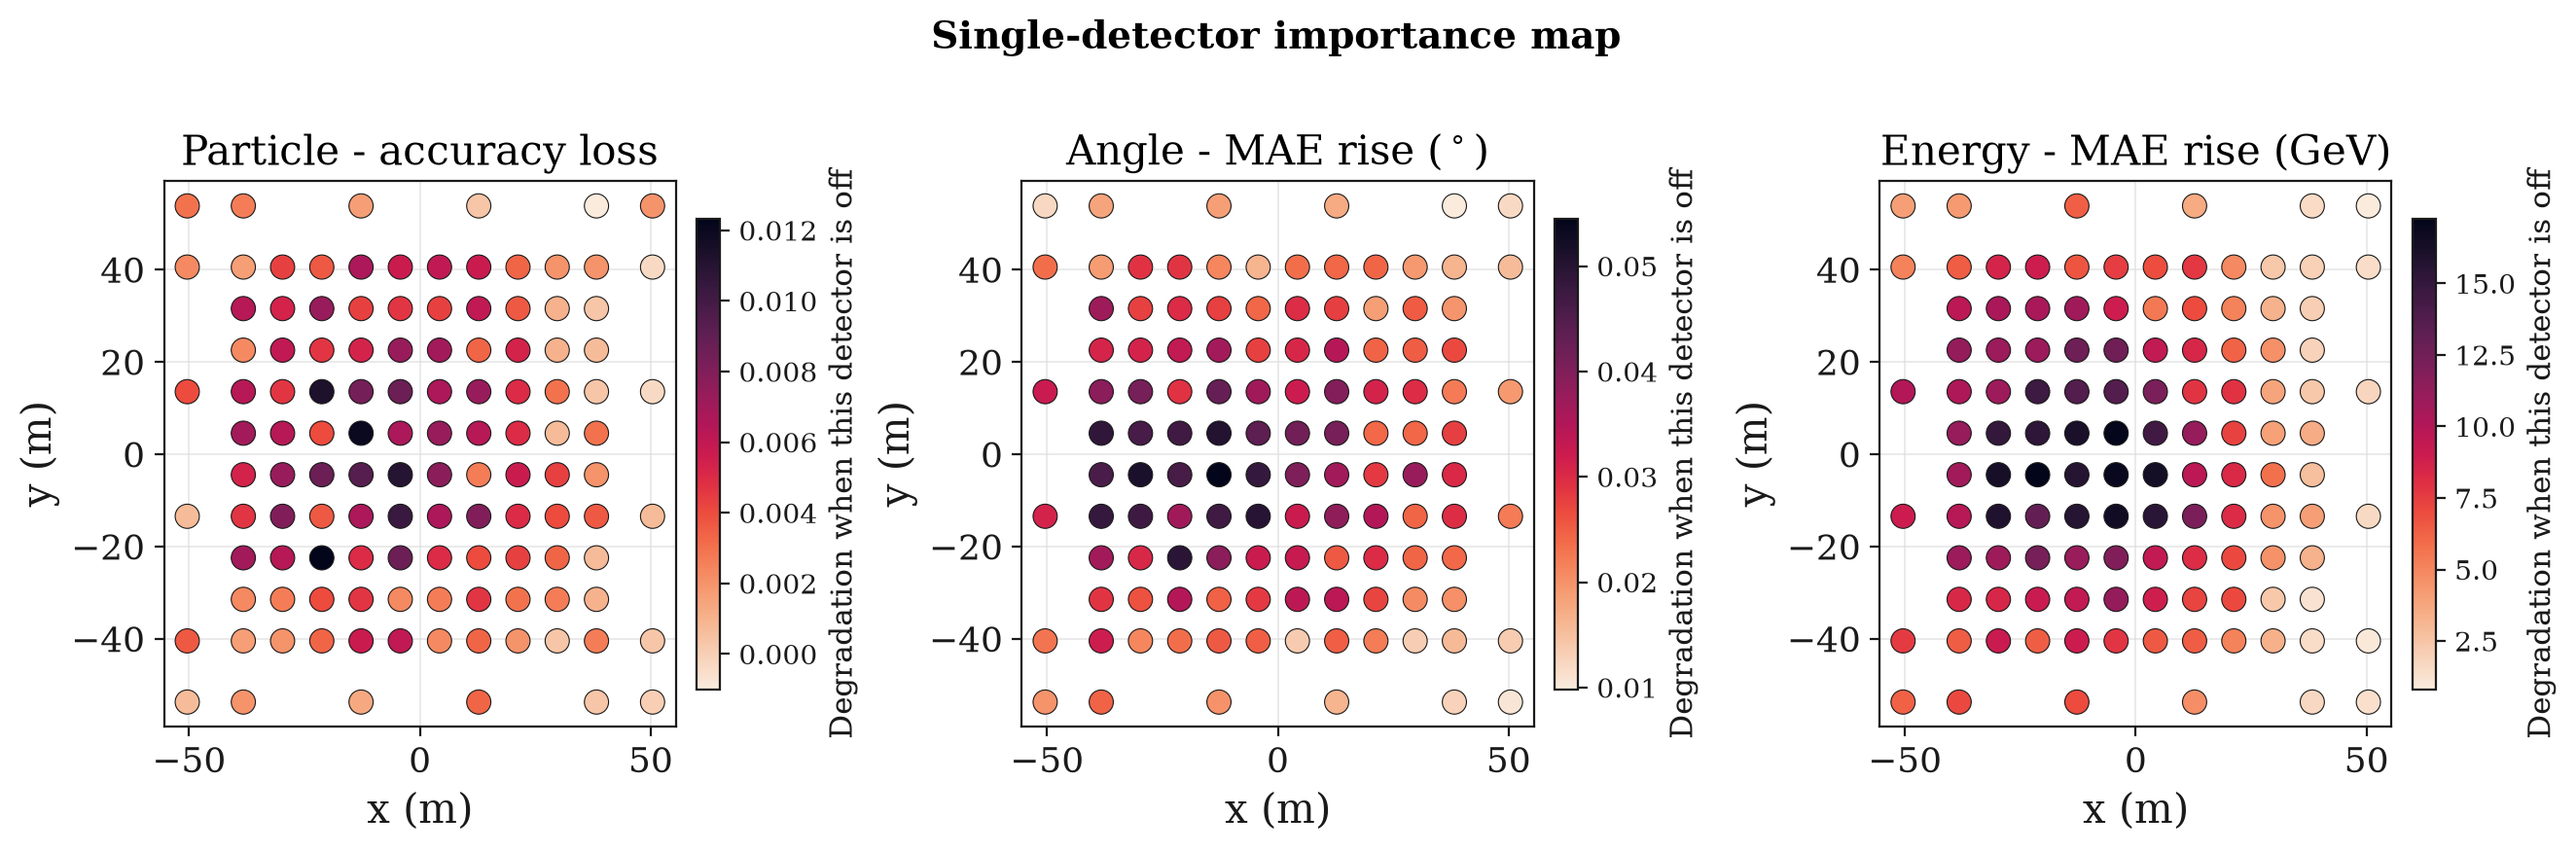
\includegraphics[width=1\linewidth]{figures/dropout_single.png}
    \caption[Single-detector importance map.]{Degradation in each task metric when each detector is individually switched off. Brighter colors indicate detectors whose loss causes the largest performance drop. The core-periphery gradient is consistent across all three tasks.}
    \label{fig:dropout_single}
\end{figure*}

\subsection{Regional Dropout}
\label{subsec:regional}

Two families of geometrically coherent detector groups are switched off simultaneously, defined in Figure~\ref{fig:dropout_regions_map}. The first follows how the array is built: the 100 modules of the central grid are split into the 36 closest to the array centre (\emph{central core}) and the 64 that surround them (\emph{outer grid}), and the 20 peripheral modules, which form a structurally separate sub-array, are kept as their own group. The second family consists of the four halves of the array, $x<0$, $x>0$, $y<0$ and $y>0$, each containing exactly 60 modules and together covering it completely.

\begin{figure}[ht!]
    \centering
    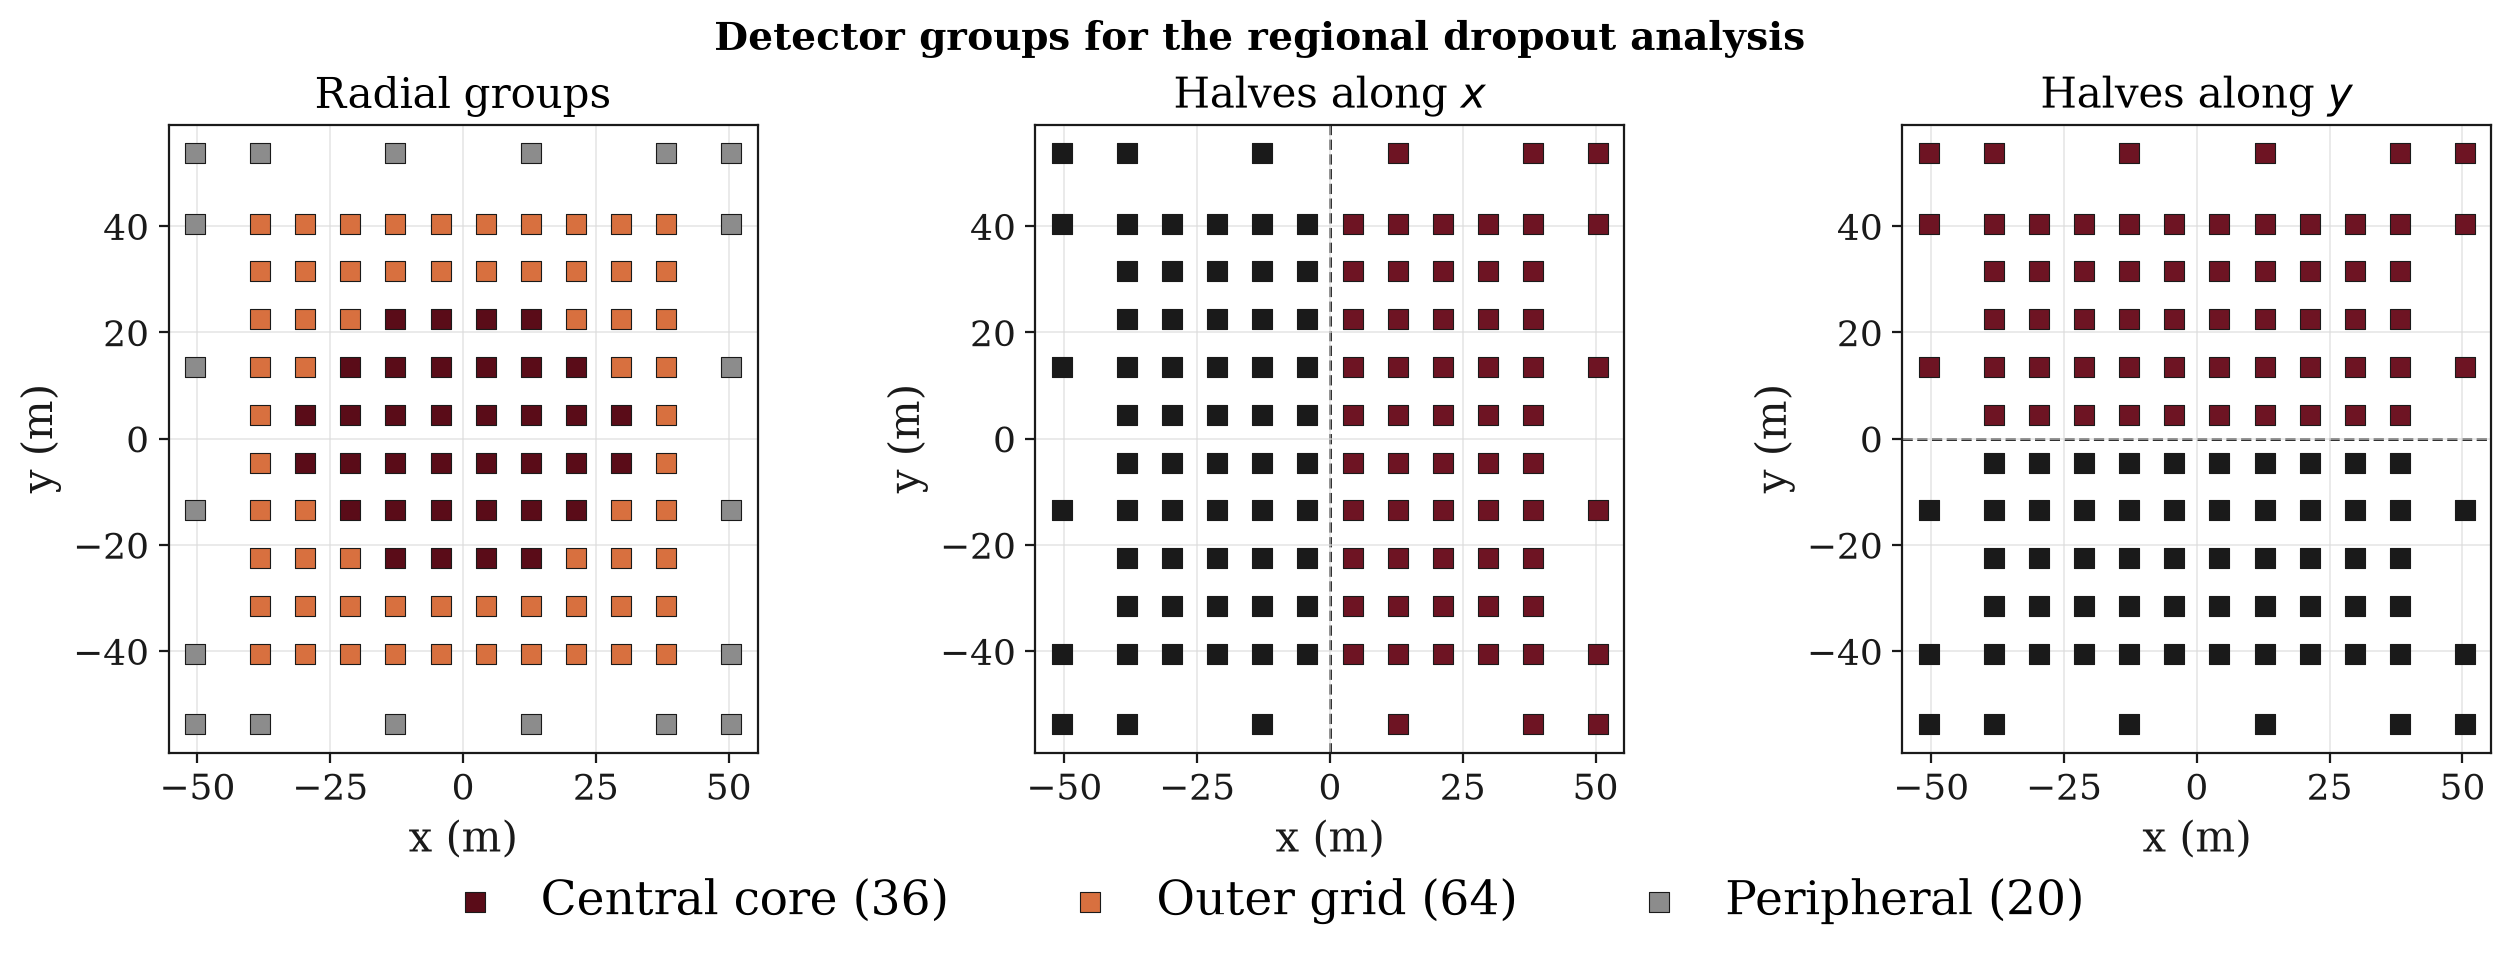
\includegraphics[width=1\linewidth]{figures/dropout_regions_map.png}
    \caption[Detector-group definitions for the regional dropout analysis.]{Spatial definition of the detector groups switched off in the regional dropout analysis. \textbf{Left:} the three radial groups --- the 36 modules closest to the array centre, the remaining 64 modules of the central grid, and the 20 peripheral modules. \textbf{Centre and right:} the four halves, split along $x$ and along $y$, of 60 modules each. The $y$ pair acts as a control for the $x$ pair: the simulated showers all arrive at azimuth $\phi = 0\degree$, which singles out the $x$ direction and should leave the $y$ halves equivalent. Marker positions correspond to the physical module locations on the array.}
    \label{fig:dropout_regions_map}
\end{figure}

Figure~\ref{fig:dropout_regional} quantifies the impact of removing each of these groups. The groups differ in size, and a larger group degrades performance more simply because it removes more detectors. Every quantity is therefore reported both as the degradation caused by removing the whole block, which corresponds to an operational failure of that block, and normalized by the number of detectors removed, which measures the contribution of an individual module. The two rankings do not coincide.

\begin{figure}[ht!]
    \centering
    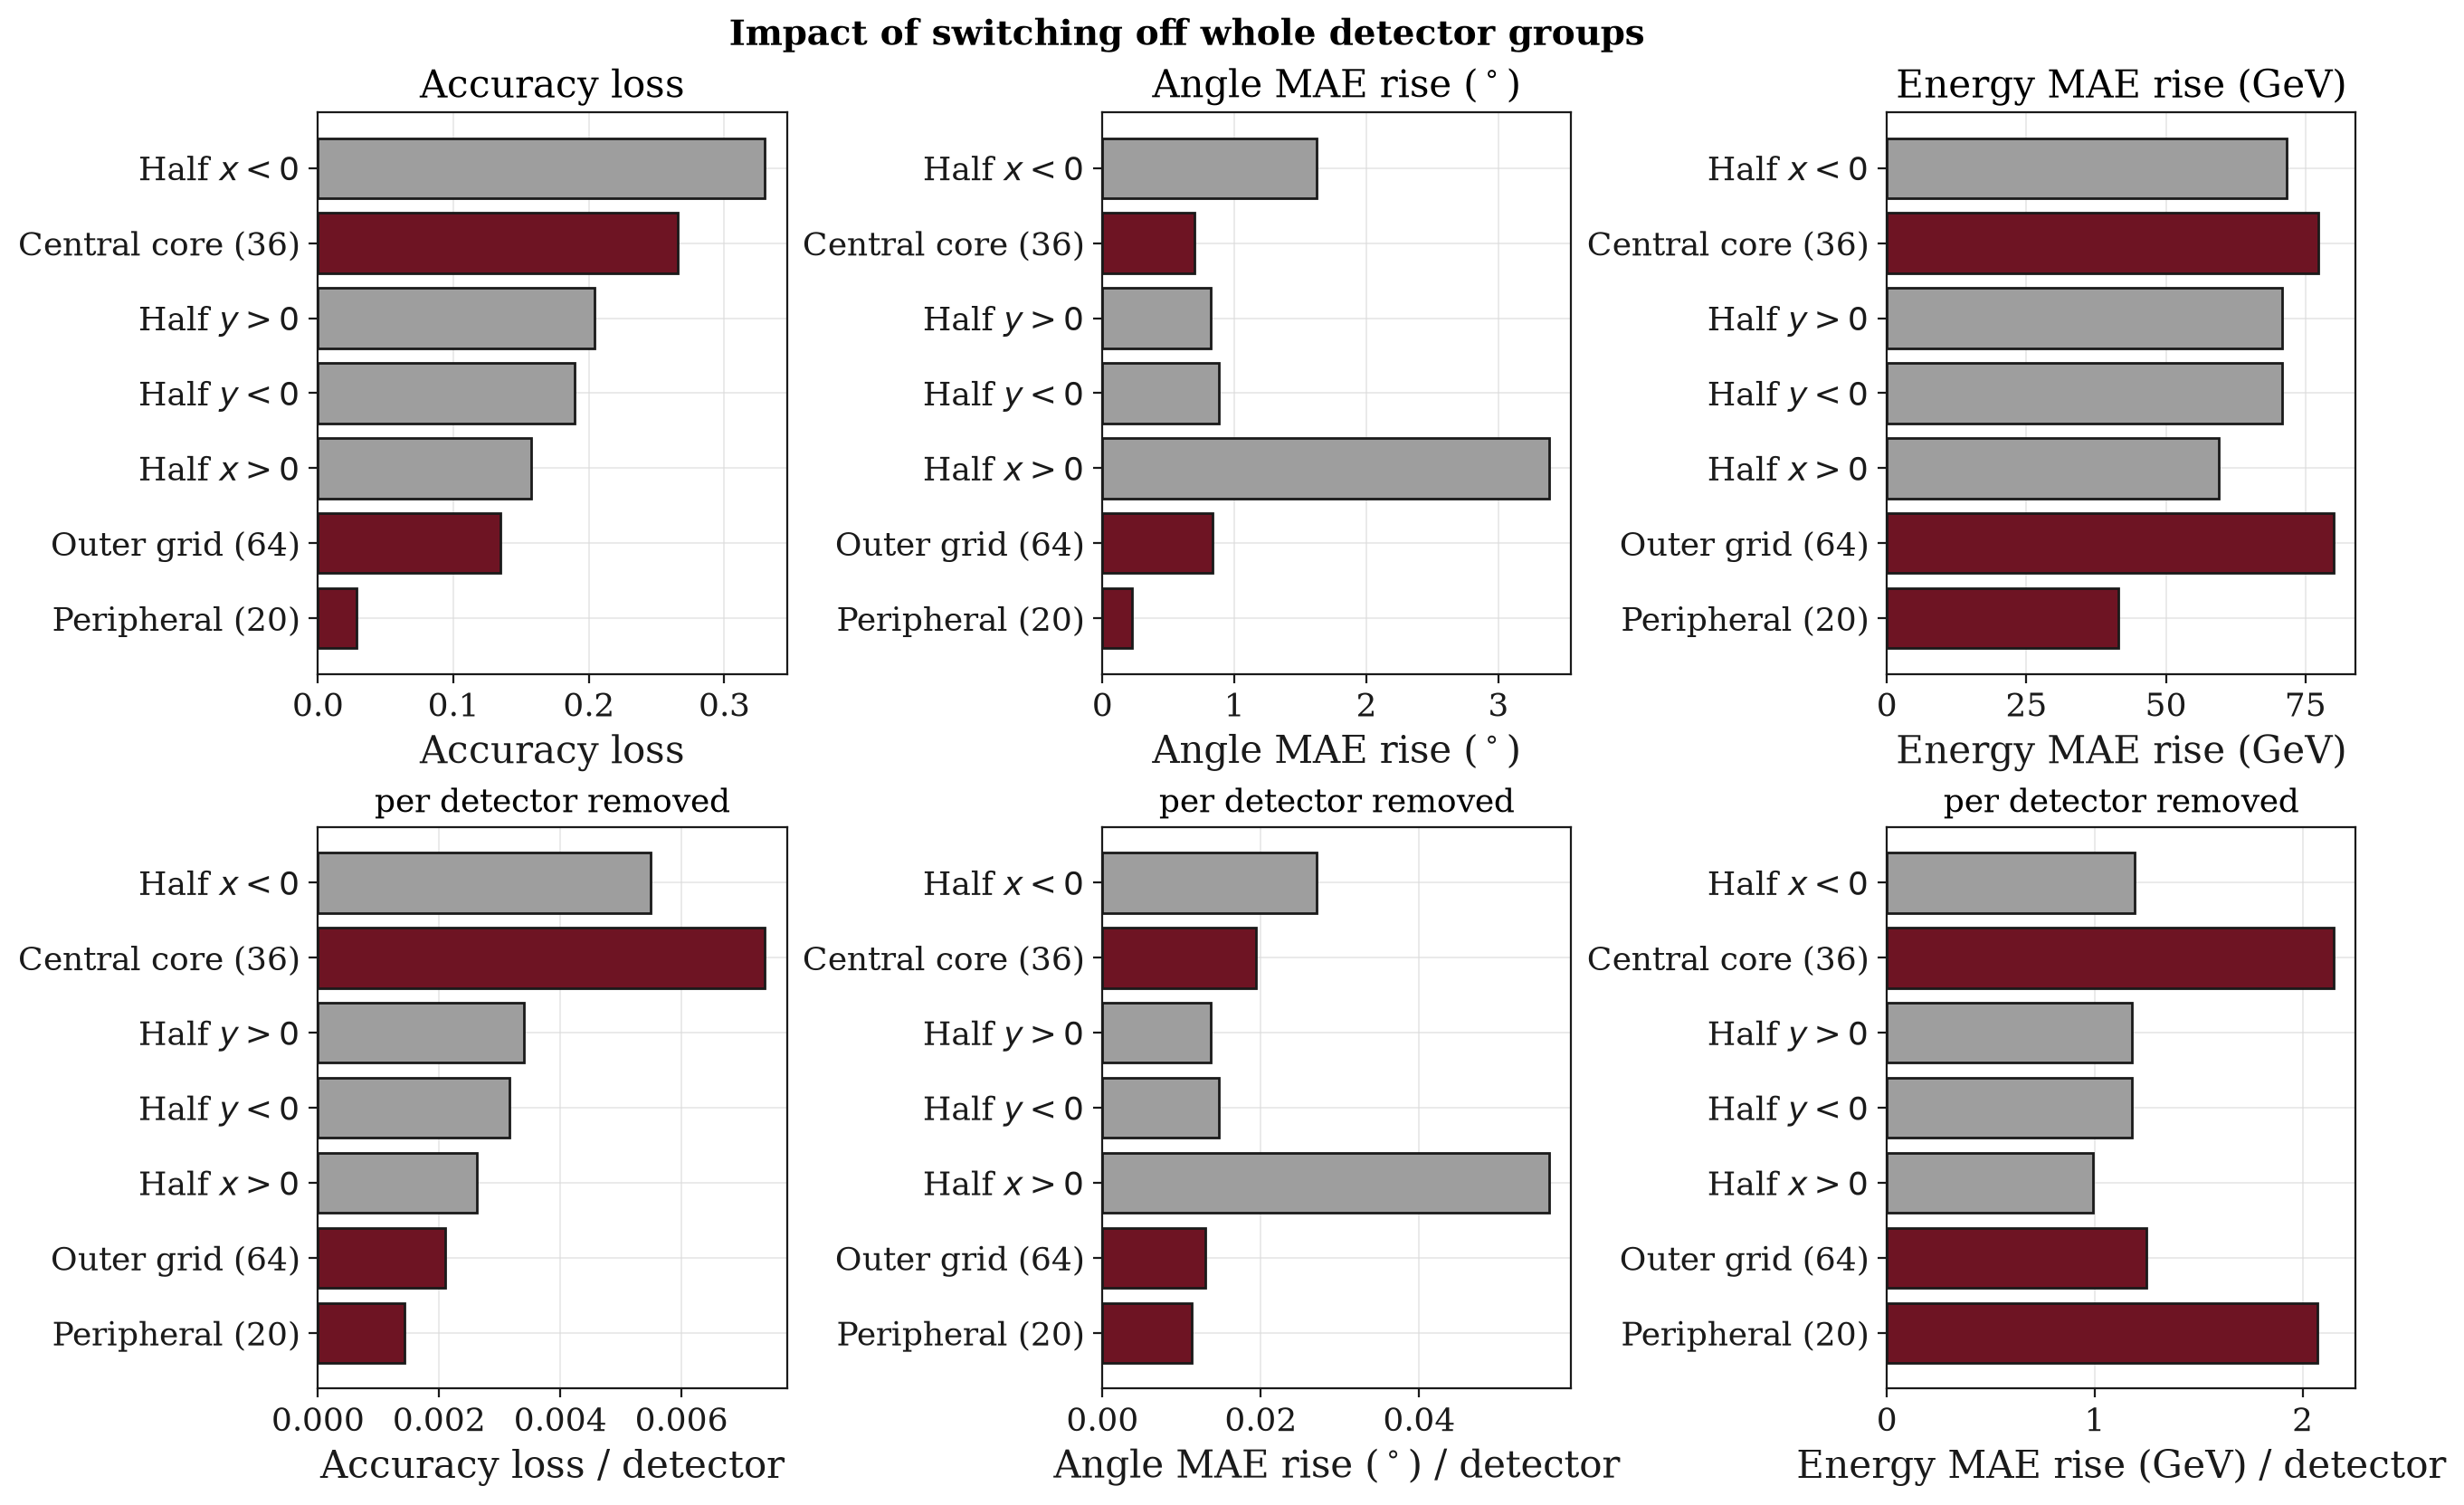
\includegraphics[width=1\linewidth]{figures/dropout_regional.png}
    \caption[Impact of switching off whole detector groups.]{Performance degradation when entire detector groups are removed, sorted by increasing impact on particle accuracy. \textbf{Top:} degradation caused by removing the whole block. \textbf{Bottom:} the same degradation per detector removed, which controls for the different group sizes. Dark red marks the three radial groups, grey the four halves.}
    \label{fig:dropout_regional}
\end{figure}

The three tasks do not depend on the same region of the array. For gamma-hadron classification the ordering follows the core-to-periphery one: removing the central core costs $0.265$ in accuracy, a relative degradation of $27.4\%$, against $13.9\%$ for the outer grid and $3.0\%$ for the 20 peripheral modules. The core achieves this while removing half as many detectors as the outer grid, so per detector it is three and a half times more damaging ($7.4 \times 10^{-3}$ against $2.1 \times 10^{-3}$ accuracy per module). Classification depends on the high particle density near the shower core, which only the central modules sample.

For angular reconstruction the ordering differs. Removing the outer grid raises the angular MAE by $0.83\degree$ ($171\%$), more than the $0.70\degree$ ($144\%$) caused by removing the central core; this is the only task for which the core is not the most damaging block. Per detector the core remains the more critical of the two ($1.9 \times 10^{-2}$ against $1.3 \times 10^{-2}$ degrees per module), so the outer grid leads as a block because it holds 64 modules against 36, but the per-detector gap is smaller than for classification. Zenith-angle recovery depends on the arrival-time gradient sampled across the lateral extent of the footprint rather than on the dense core alone, so the spatial spread of the modules contributes almost as much as their density.

For energy reconstruction the two normalizations disagree. In absolute terms the peripheral modules are the least important group ($+41$~GeV, $38.9\%$, against $+77$ and $+80$~GeV for the core and the outer grid). Per detector removed they are almost as costly as the central core ($2.07$ against $2.15$~GeV per module) and above the outer grid ($1.25$~GeV). The 20 outermost modules are therefore not redundant for energy estimation: each contributes approximately as much as a core module, and their low block-level ranking reflects their small number. This is consistent with energy estimation requiring the lateral extent of the shower to be sampled, and with the sparsification results of Section~\ref{subsec:count_layout}.

\textbf{Azimuthal dependence.} The $y$ pair acts as a control and shows no asymmetry: removing $y<0$ or $y>0$ gives essentially the same degradation in all three tasks (accuracy $19.6\%$ vs $21.1\%$, angular MAE $+0.88\degree$ vs $+0.82\degree$, energy $+70.8$~GeV in both cases). The $x$ pair, by contrast, is strongly asymmetric, and in opposite directions depending on the task: for classification the $x<0$ half is more than twice as damaging as $x>0$ ($34.1\%$ vs $16.3\%$), whereas for angular reconstruction the ordering reverses and $x>0$ is by far the more critical, raising the MAE by $3.38\degree$ against $1.63\degree$. The two directions are geometrically equivalent in the array, so the asymmetry originates in the dataset: all showers arrive at a fixed azimuth $\phi = 0\degree$, an inclined shower is therefore always displaced along the same direction in $x$, and the two $x$ halves sample systematically different parts of the footprint, with the trailing side carrying most of the arrival-time information on which the zenith angle depends. The agreement of the $y$ pair indicates that the procedure introduces no directional bias of its own, so the $x$ asymmetry is a property of the simulation configuration rather than of the array; a dataset with uniformly sampled azimuth would be expected to make both pairs symmetric.

\subsection{Detector Count and Layout}
\label{subsec:count_layout}


The preceding subsections quantified which detectors the model depends on. This subsection addresses the number of detectors required and the way they are distributed over the ground, which together define an array configuration. Both are evaluated with the same switch-off procedure: the number by removing detectors at random and increasing the removed fraction, the distribution by comparing different ways of removing the same number of detectors.

\textbf{Progressive random failure.} Figure~\ref{fig:dropout_progressive} shows the degradation of each task metric as an increasing fraction of randomly chosen detectors is switched off, averaged over four independent random subsets per fraction level. This measures the failure rate the array can absorb before reconstruction degrades appreciably.

\begin{figure*}[ht!]
    \centering
    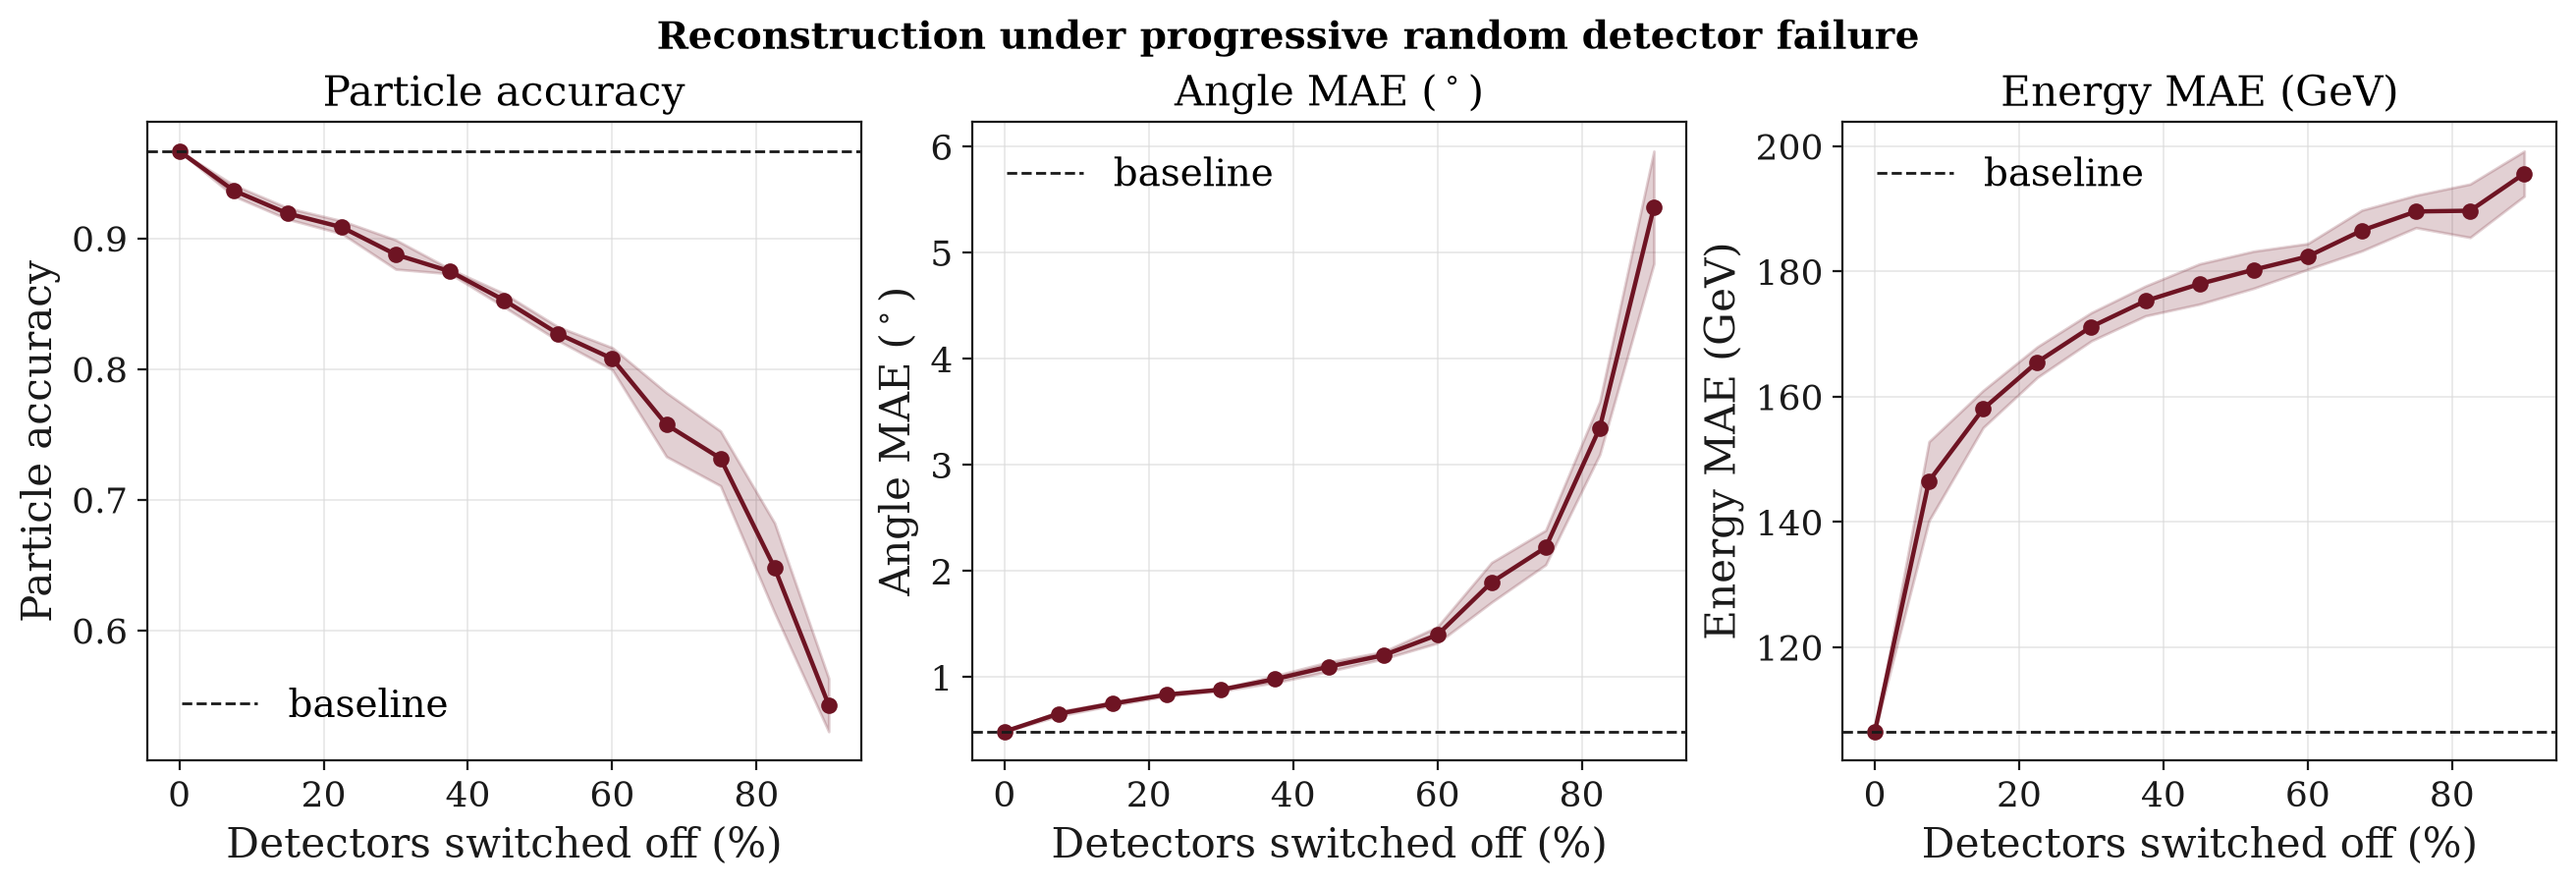
\includegraphics[width=1\linewidth]{figures/dropout_progressive.png}
    \caption[Reconstruction under progressive random detector failure.]{Task metric as a function of the fraction of detectors switched off at random. Shaded bands indicate one standard deviation over four random subsets per fraction. Dashed horizontal lines indicate baseline performance with all detectors active.}
    \label{fig:dropout_progressive}
\end{figure*}

Gamma-hadron classification is the most fault-tolerant task: accuracy stays above $90\%$ with up to about $22\%$ of the detectors offline and above $85\%$ up to roughly $45\%$, collapsing more steeply only beyond ${\sim}60\%$ loss.

The angular and energy reconstruction tasks begin to degrade more immediately. Angular MAE grows steadily, roughly doubling from its $0.49\degree$ baseline to ${\sim}1.0\degree$ at about $45\%$ detector loss and rising sharply thereafter. Energy MAE increases quickly at first --- from $107$~GeV to ${\sim}171$~GeV by $30\%$ loss --- and then saturates near $185$--$195$~GeV, a plateau that reflects the model falling back toward predicting the mean energy of the range once too few detectors survive to constrain the shower size.

This difference in fault tolerance reflects the nature of each task: binary classification can exploit redundant evidence across many detectors and remains viable as long as some discriminative detectors survive, while metric regression requires information from a spatially distributed set of detectors to triangulate the shower geometry and measure its total energy. The knee in the particle-accuracy curve near $60$--$70\%$ corresponds to the point at which too few spatially distinct measurements survive to resolve the shower footprint.

\textbf{Layout at matched detector count.} Random thinning reduces the detector count while leaving the covered area unchanged, so it does not separate the effect of the number of detectors from that of their arrangement. Figure~\ref{fig:dropout_geometry} compares three ways of reaching the same count: random thinning (detectors removed uniformly at random, sparser over the same area), central crop (only detectors within a shrinking radius are retained, denser over a smaller area), and a checkerboard pattern (every other detector removed, approximately halving the count while maintaining full coverage). At equal detector count, the differences between the three curves are attributable to the arrangement alone.

\begin{figure*}[ht!]
    \centering
    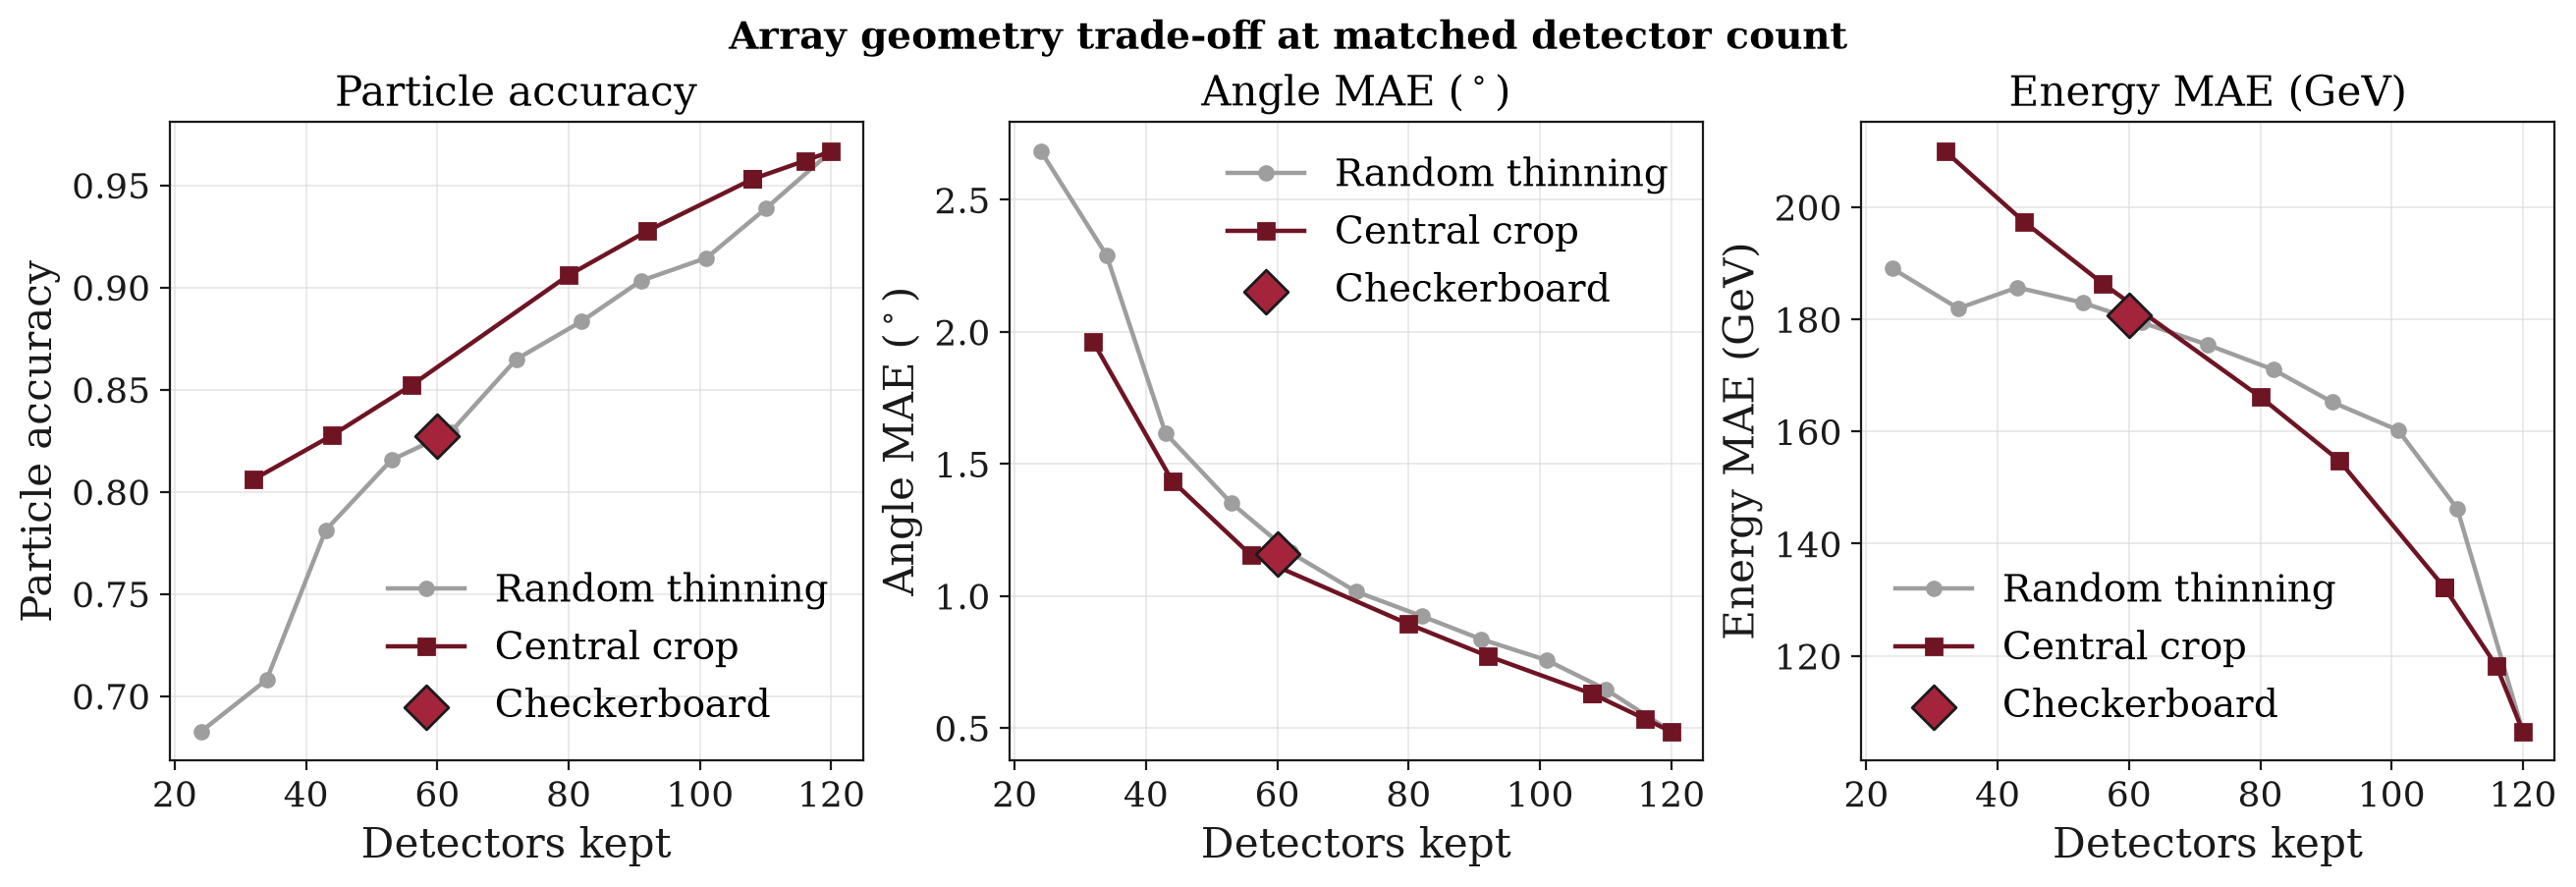
\includegraphics[width=1\linewidth]{figures/dropout_geometry.png}
    \caption[Array geometry trade-off at matched detector counts.]{Reconstruction performance as a function of the number of active detectors, for three sparsification strategies. Central crop (denser, smaller array) outperforms random thinning (sparser, same area) at equal detector count for classification and angular reconstruction; for energy the central crop wins only above ${\sim}65$ detectors and random thinning is better below that. The checkerboard point (diamond) corresponds to approximately 60 active detectors.}
    \label{fig:dropout_geometry}
\end{figure*}

The central crop strategy outperforms random thinning at matched detector counts for gamma-hadron classification and angular reconstruction at every count tested: for these two tasks, retaining the detectors closest to the array centre yields better reconstruction than retaining a random subset distributed over the full array area. Energy reconstruction, however, behaves differently. At high detector counts the central crop still performs better, but below roughly 65 active detectors the ordering reverses and random thinning gives the lower energy MAE. This crossover is consistent with the per-detector result of Section~\ref{subsec:regional}, where the peripheral modules were found to be nearly as valuable per unit as the core modules for energy: energy estimation relies on sampling the lateral extent of the shower, so under aggressive thinning a wide but sparse layout preserves outer footprint information that a dense central cluster discards. The checkerboard pattern (about 60 active detectors) falls close to the random-thinning curve for all three tasks, and in particular sits near this energy crossover, performing comparably to random thinning while remaining inferior to the central crop for classification and angular reconstruction.

Taken across the three studies, the results point in a consistent direction. Classification and angular reconstruction degrade least under the central crop, favouring a denser core; energy reconstruction follows the lateral spread of the modules instead and, below roughly 65 active detectors, favours a wide sparse layout over a dense central cluster. A dedicated study of the array layout, including geometries outside the present family such as hexagonal grids, variable pitch, or elliptical footprints, would re-run the CORSIKA pipeline and retrain the model for each configuration, and is left for future work.